\documentclass[journal]{IEEEtran}
\usepackage[a5paper, margin=10mm]{geometry}
\usepackage{tfrupee} % Include tfrupee package

\setlength{\headheight}{1cm} % Set the height of the header box
\setlength{\headsep}{0mm}     % Set the distance between the header box and the top of the text

\usepackage{gvv-book}
\usepackage{gvv}
\usetikzlibrary{patterns}
\lstset{aboveskip=12pt}
\usepackage[center]{caption}
\raggedbottom
\hypersetup{
    colorlinks=true,
    urlcolor=black % Changes text color instead of placing a box around it
}
\usepackage{amsfonts}
\makeindex

\begin{document}
\bibliographystyle{IEEEtran}
\onecolumn

\title{CBSE Class 12 - 2018 Mathematics\\Question Papers\\
\large Math for EE\\[-0.5em]
\rule{0.4\columnwidth}{0.4pt}
}

\author{Vishweshwar - ee26btech11225
\vspace{10cm}
\begin{center}
    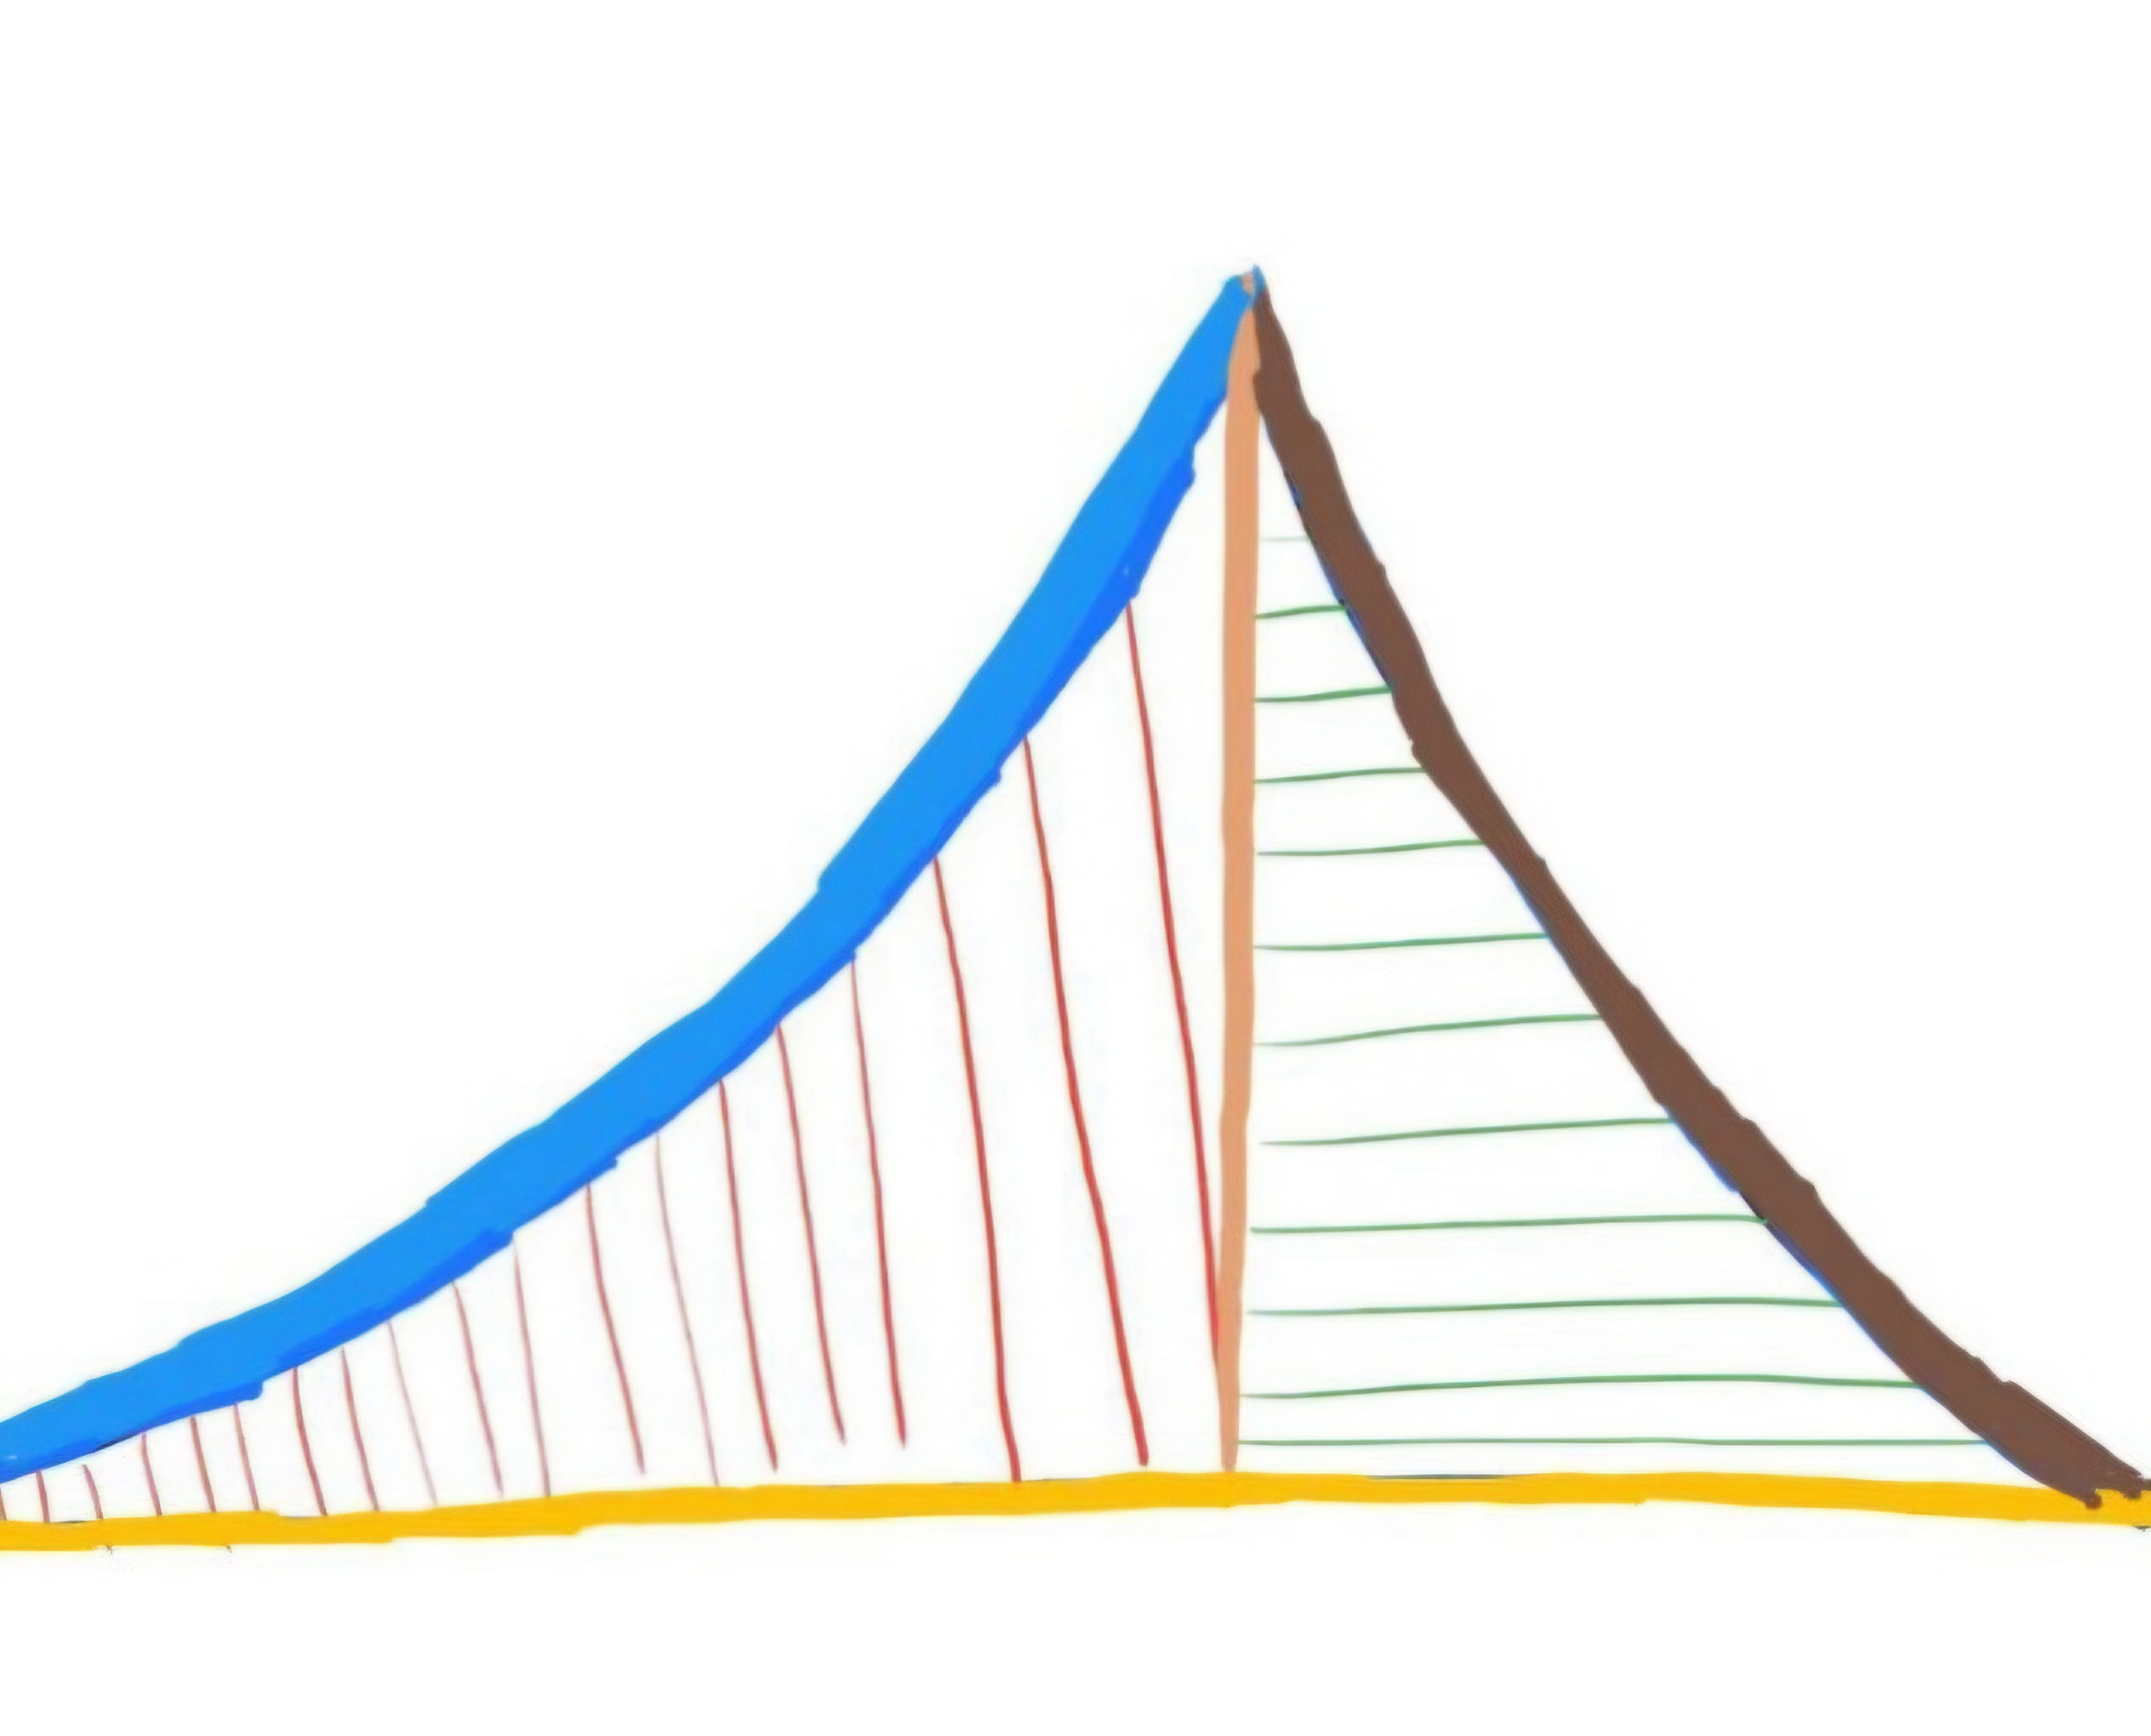
\includegraphics[width=0.2\columnwidth]{figs/logo.jpg}\\
    {\huge G. V. V. Sharma}
\end{center}
}

\maketitle
\newpage

\section*{About this Book}
This document contains the unique questions from the CBSE Class 12 Mathematics question paper sets being studied (currently Code 65/5/2, Series BVM/5, SET-2).

Questions are typed in their original wording, with the original options and diagrams wherever applicable.

Where the same question appears in multiple sets, it will be included only once, provided the wording, values, options, and diagrams are identical.

The Python programs in the \texttt{codes} folder use the \texttt{CoordGeo} library and verify every solution; they also generate the figures in this book.

\newpage
\tableofcontents
\newpage
\onecolumn

\numberwithin{equation}{enumi}
\numberwithin{figure}{enumi}
\renewcommand{\thetable}{\theenumi}

\section{CBSE CLASS-12 MATH 2018}
\subsection{Formulae}
\begin{enumerate}[label=\thesubsection.\arabic*, ref=\thesubsection.\theenumi]

    \item Determinant properties for a square matrix $A$ of order $n$ and a scalar $k$:
\begin{align}
    |AB| = |A||B|, \quad |A'| = |A|, \quad |kA| = k^n |A| \label{eq:EE26BTECH11225-det}
\end{align}

    \item Inverse trigonometric identities:
\begin{align}
    \cos^{-1}(\cos t) &= t, \quad t \in [0,\pi] \label{eq:EE26BTECH11225-invtrig-1} \\
    \tan^{-1}a + \tan^{-1}b &= \tan^{-1}\frac{a+b}{1-ab}, \quad ab < 1 \label{eq:EE26BTECH11225-invtrig-2} \\
    \tan^{-1}x + \cot^{-1}x &= \frac{\pi}{2} \label{eq:EE26BTECH11225-invtrig-3} \\
    \sin^{-1}x &= \tan^{-1}\frac{x}{\sqrt{1-x^2}}, \quad |x|<1 \label{eq:EE26BTECH11225-invtrig-4}
\end{align}

    \item Angle $\theta$ between a line with direction vector $\vec{b}$ and a plane with normal vector $\vec{n}$:
\begin{align}
    \sin\theta = \frac{|\vec{b}^{\top}\vec{n}|}{\|\vec{b}\|\,\|\vec{n}\|} \label{eq:EE26BTECH11225-lineplane}
\end{align}

    \item For vectors $\vec{a}$, $\vec{b}$ with angle $\theta$ between them:
\begin{align}
    \vec{a}^{\top}\vec{b} &= \|\vec{a}\|\|\vec{b}\|\cos\theta \label{eq:EE26BTECH11225-dot} \\
    \|\vec{a}\times\vec{b}\| &= \|\vec{a}\|\|\vec{b}\|\sin\theta \label{eq:EE26BTECH11225-cross}
\end{align}

    \item A binary operation $*$ on a set $S$ requires $a*b \in S$ for all $a,b\in S$ (closure). It is commutative if
\begin{align}
    a*b = b*a \quad \forall\, a,b \in S \label{eq:EE26BTECH11225-binop}
\end{align}

    \item Binomial probability for $n$ independent trials with success probability $p$ ($q=1-p$), and independent events:
\begin{align}
    P(X=k) &= \binom{n}{k}p^k q^{n-k} \label{eq:EE26BTECH11225-binom} \\
    P(A\cap B) &= P(A)P(B) \label{eq:EE26BTECH11225-indep} \\
    P(A'\cap B') &= \big(1-P(A)\big)\big(1-P(B)\big) \label{eq:EE26BTECH11225-indep-comp}
\end{align}
Probability that exactly one of $A$, $B$ occurs:
\begin{align}
    P(A)P(B') + P(A')P(B) \label{eq:EE26BTECH11225-exactly-one}
\end{align}

    \item First order linear differential equation and its integrating factor:
\begin{align}
    \frac{dy}{dx} + P(x)y = Q(x), \quad \text{I.F.} = e^{\int P\,dx}, \quad y\cdot\text{I.F.} = \int Q\cdot\text{I.F.}\,dx + C \label{eq:EE26BTECH11225-linode}
\end{align}

    \item Homogeneous differential equation: substitute $y = vx$,
\begin{align}
    \frac{dy}{dx} = v + x\frac{dv}{dx} \label{eq:EE26BTECH11225-homog}
\end{align}

    \item Differential equation of a family of curves with $n$ arbitrary constants: differentiate $n$ times and eliminate the constants. \label{eq:EE26BTECH11225-family}

    \item Points $A, B, C$ are collinear if $\vec{BC} = k\,\vec{AB}$. Points $A,B,C,D$ are coplanar if
\begin{align}
    \det\begin{bmatrix}\vec{AB} & \vec{AC} & \vec{AD}\end{bmatrix} = 0 \label{eq:EE26BTECH11225-coplanar}
\end{align}

    \item Standard integrals:
\begin{align}
    \int e^x\big[f(x)+f'(x)\big]dx &= e^x f(x) + C \label{eq:EE26BTECH11225-expint} \\
    \int \frac{du}{\sqrt{a^2-u^2}} &= \sin^{-1}\frac{u}{a} + C \label{eq:EE26BTECH11225-sininv} \\
    \int \sqrt{a^2-u^2}\,du &= \frac{u}{2}\sqrt{a^2-u^2} + \frac{a^2}{2}\sin^{-1}\frac{u}{a} + C \label{eq:EE26BTECH11225-sqrtint} \\
    2\cos A\cos B &= \cos(A+B) + \cos(A-B) \label{eq:EE26BTECH11225-prodsum}
\end{align}
\textbf{Proof of (\ref{eq:EE26BTECH11225-expint}):} By parts, $\int e^x f\,dx = e^x f - \int e^x f'\,dx$; rearranging gives the result.

    \item A plane through a point $\vec{P}_0$ with normal $\vec{n}$ is $\vec{n}^{\top}(\vec{x}-\vec{P}_0)=0$. A plane perpendicular to two planes with normals $\vec{n}_1,\vec{n}_2$ has normal
\begin{align}
    \vec{n} = \vec{n}_1\times\vec{n}_2 \label{eq:EE26BTECH11225-plane}
\end{align}

    \item Integral of a modulus function: split the interval at the points where each expression changes sign, e.g.
\begin{align}
    \int_a^b |x-c|\,dx = \int_a^c (c-x)\,dx + \int_c^b (x-c)\,dx, \quad a<c<b \label{eq:EE26BTECH11225-absint}
\end{align}

    \item Inverse of a matrix and elementary row operations:
\begin{align}
    A^{-1} &= \frac{1}{|A|}\,\text{adj}(A), \quad |A|\neq 0 \label{eq:EE26BTECH11225-adj} \\
    \big[A \,|\, I\big] &\xrightarrow{\text{row operations}} \big[I \,|\, A^{-1}\big] \label{eq:EE26BTECH11225-rowops}
\end{align}
A system $A\vec{x}=\vec{b}$ with $|A|\neq0$ has the unique solution $\vec{x}=A^{-1}\vec{b}$.

    \item A relation is an equivalence relation if it is reflexive, symmetric and transitive. A function is invertible if it is one-one and onto. \label{eq:EE26BTECH11225-equiv}

    \item Logarithmic differentiation of $y = u(x)^{v(x)}$:
\begin{align}
    \ln y = v\ln u \implies \frac{1}{y}\frac{dy}{dx} = v'\ln u + \frac{v\,u'}{u} \label{eq:EE26BTECH11225-logdiff}
\end{align}

    \item If $f'(x)<0$ on an interval, then $f$ is strictly decreasing on that interval. At a critical point $f'(x)=0$, if $f''(x)<0$ then $f$ has a maximum. \label{eq:EE26BTECH11225-mono}

    \item Area between two curves and area of a triangle with vertices $A,B,C$:
\begin{align}
    \text{Area} &= \int_a^b \big[y_1(x)-y_2(x)\big]dx \label{eq:EE26BTECH11225-area-curves} \\
    \text{Area} &= \int_c^d \big[x_1(y)-x_2(y)\big]dy \label{eq:EE26BTECH11225-area-curves-y} \\
    \text{Area}(\Delta ABC) &= \frac{1}{2}\Big|\det\begin{bmatrix}B-A & C-A\end{bmatrix}\Big| \label{eq:EE26BTECH11225-area-tri}
\end{align}

    \item Distance between parallel lines $\vec{x}=\vec{a}_1+\lambda\vec{b}$ and $\vec{x}=\vec{a}_2+\mu\vec{b}$:
\begin{align}
    d = \frac{\|(\vec{a}_2-\vec{a}_1)\times\vec{b}\|}{\|\vec{b}\|} \label{eq:EE26BTECH11225-distance-lines}
\end{align}
Foot of the perpendicular from $\vec{P}$ to the plane $\vec{n}^{\top}\vec{x}=c$ and the image of $\vec{P}$:
\begin{align}
    \vec{Q} = \vec{P}+t\vec{n}, \quad t = \frac{c-\vec{n}^{\top}\vec{P}}{\|\vec{n}\|^2}, \quad \vec{P}' = \vec{P}+2t\vec{n} \label{eq:EE26BTECH11225-foot}
\end{align}

    \item Linear programming: the optimum of a linear objective over a convex feasible region occurs at a corner point.
\begin{align}
    \max Z = \vec{c}^{\top}\vec{x} \quad \text{s.t.}\quad A\vec{x}\leq\vec{b},\; \vec{x}\geq\vec{0} \label{eq:EE26BTECH11225-lpp}
\end{align}

    \item Bayes' theorem:
\begin{align}
    P(E_1|A) = \frac{P(E_1)P(A|E_1)}{P(E_1)P(A|E_1)+P(E_2)P(A|E_2)} \label{eq:EE26BTECH11225-bayes}
\end{align}

    \item Cylinder inscribed in a cone of base radius $R$ and height $H$: if the cylinder has radius $r$ and height $h$, similar triangles give
\begin{align}
    h = \frac{H(R-r)}{R}, \quad \text{CSA} = 2\pi r h \label{eq:EE26BTECH11225-inscribed}
\end{align}

\end{enumerate}

\subsection{Problems}
\begin{enumerate}[label=\thesubsection.\arabic*, ref=\thesubsection.\theenumi]

    \item If $A$ is a square matrix of order 2 and $|A| = 4$, then find the value of $|2 \cdot AA'|$, where $A'$ is the transpose of matrix $A$.

\solution From \eqref{eq:EE26BTECH11225-det} with $n=2$ and $k=2$:
\begin{align}
    |2 \cdot AA'| &= 2^2 |AA'| \\
    &= 4|A||A'| = 4|A|^2 \\
    &= 4(4)^2 = 64
\end{align}

    \item
    \begin{enumerate}[label=(\alph*), leftmargin=1.5em, labelsep=0.5em]
        \item Find the angle between the line $\vec{r} = (2\hat{i} - \hat{j} + 3\hat{k}) + \lambda(3\hat{i} - \hat{j} + 2\hat{k})$ and the plane $\vec{r}\cdot(\hat{i}+\hat{j}+\hat{k}) = 3$.

        \begin{center}
            \textbf{OR}
        \end{center}

        \item Find the co-ordinates of the point, where the line $\dfrac{x+2}{1} = \dfrac{y-5}{3} = \dfrac{z+1}{5}$ cuts the $yz$-plane.
    \end{enumerate} \vspace{2pt}
    \textbf{(a) Solution:} The direction vector of the line and the normal of the plane are
\begin{align}
    \vec{b} = \myvec{3 \\ -1 \\ 2}, \quad \vec{n} = \myvec{1 \\ 1 \\ 1}
\end{align}
From \eqref{eq:EE26BTECH11225-lineplane}:
\begin{align}
    \sin\theta &= \frac{|(3)(1)+(-1)(1)+(2)(1)|}{\sqrt{3^2+(-1)^2+2^2}\sqrt{1^2+1^2+1^2}} \\
    &= \frac{4}{\sqrt{14}\sqrt{3}} = \frac{4}{\sqrt{42}} \\
    &\implies \theta = \sin^{-1}\left(\frac{4}{\sqrt{42}}\right) \approx 38.11^\circ
\end{align}
\textbf{(b) Solution:} On the $yz$-plane $x = 0$. Let the common ratio be $\lambda$:
\begin{align}
    \frac{0+2}{1} = \lambda = 2 &\implies y - 5 = 3(2) \implies y = 11 \\
    &\implies z + 1 = 5(2) \implies z = 9
\end{align}
Thus, the point is $(0, 11, 9)$. The following code verifies both parts and generates \figref{fig:lineplane_q2}.
\begin{lstlisting}[frame=single, basicstyle=\rmfamily, escapeinside={(*@}{@*)}]
(*@\makebox[\dimexpr\linewidth-2\fboxsep-2\fboxrule\relax][c]{codes/LinePlane.py}@*)
\end{lstlisting}
\begin{figure}[H]
    \centering
    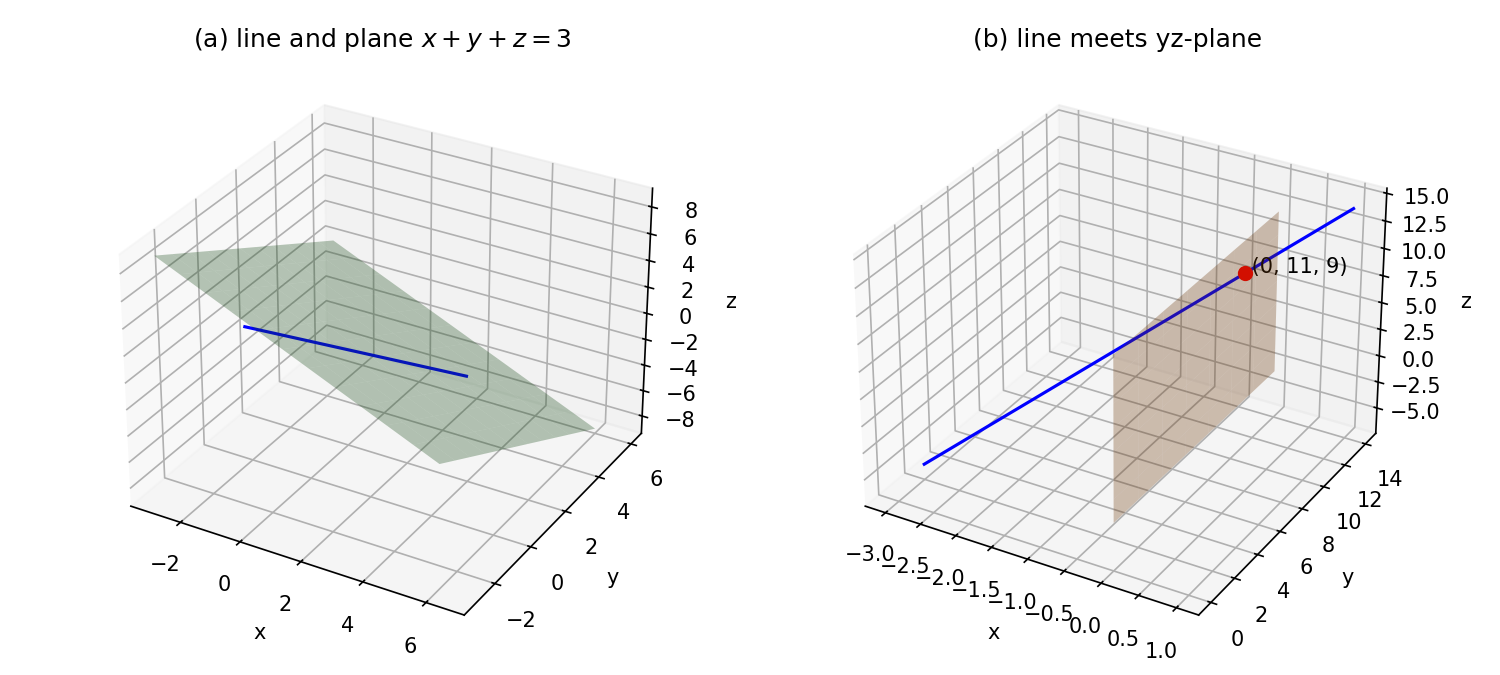
\includegraphics[width=0.95\linewidth]{figs/LinePlane.png}
    \caption{(a) Line and plane $x+y+z=3$; (b) line meeting the $yz$-plane at $(0,11,9)$}
    \label{fig:lineplane_q2}
\end{figure}

    \item Find the differential equation representing the family of curves $y = -A\cos 3x + B\sin 3x$.

\solution The family has two arbitrary constants $A$ and $B$, so by \ref{eq:EE26BTECH11225-family} we differentiate twice:
\begin{align}
    \frac{dy}{dx} &= 3A\sin 3x + 3B\cos 3x \\
    \frac{d^2y}{dx^2} &= 9A\cos 3x - 9B\sin 3x = -9\left(-A\cos 3x + B\sin 3x\right) = -9y
\end{align}
Hence the differential equation is
\begin{align}
    \frac{d^2y}{dx^2} + 9y = 0
\end{align}
The following code verifies this symbolically and plots members of the family in \figref{fig:odefamily_q3}.
\begin{lstlisting}[frame=single, basicstyle=\rmfamily, escapeinside={(*@}{@*)}]
(*@\makebox[\dimexpr\linewidth-2\fboxsep-2\fboxrule\relax][c]{codes/OdeFamily.py}@*)
\end{lstlisting}
\begin{figure}[H]
    \centering
    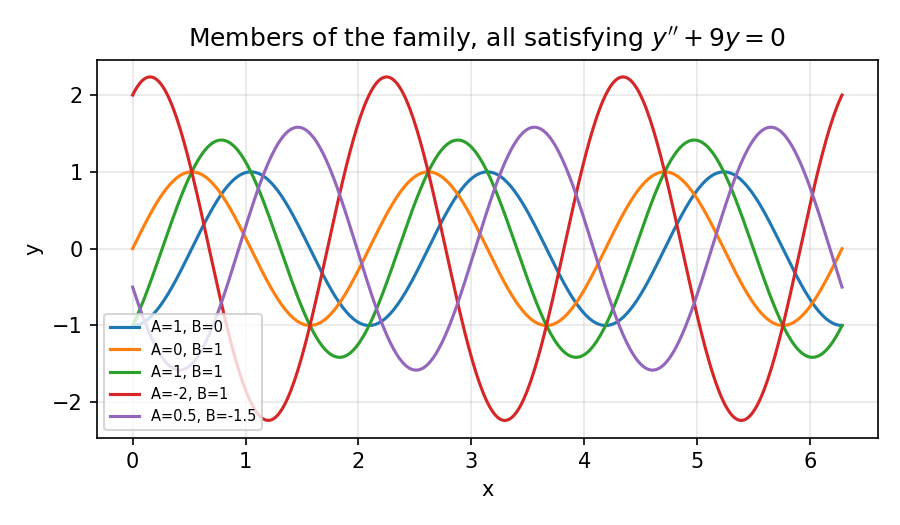
\includegraphics[width=0.75\linewidth]{figs/OdeFamily.png}
    \caption{Members of the family $y=-A\cos 3x+B\sin 3x$}
    \label{fig:odefamily_q3}
\end{figure}

    \item Find the differential of the function $\cos^{-1}(\sin 2x)$ w.r.t. $x$.

\solution Since $\sin 2x = \cos\left(\frac{\pi}{2} - 2x\right)$, from \eqref{eq:EE26BTECH11225-invtrig-1}, for $\frac{\pi}{2}-2x \in [0,\pi]$, i.e. $-\frac{\pi}{4}\leq x\leq\frac{\pi}{4}$:
\begin{align}
    y &= \cos^{-1}\left(\cos\left(\frac{\pi}{2}-2x\right)\right) = \frac{\pi}{2} - 2x \\
    &\implies \frac{dy}{dx} = -2
\end{align}
The following code verifies the derivative numerically and plots \figref{fig:invtrig_q4}.
\begin{lstlisting}[frame=single, basicstyle=\rmfamily, escapeinside={(*@}{@*)}]
(*@\makebox[\dimexpr\linewidth-2\fboxsep-2\fboxrule\relax][c]{codes/InvTrig.py}@*)
\end{lstlisting}
\begin{figure}[H]
    \centering
    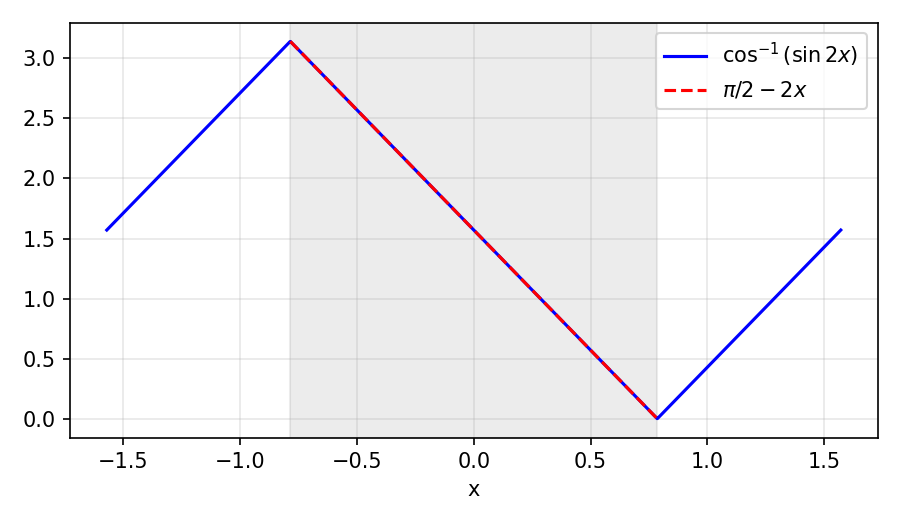
\includegraphics[width=0.70\linewidth]{figs/InvTrig.png}
    \caption{Plot of $\cos^{-1}(\sin 2x)$; it is the line $\frac{\pi}{2}-2x$ on the shaded region}
    \label{fig:invtrig_q4}
\end{figure}

    \item If an operation $*$ on the set of integers $\mathbb{Z}$ is defined by $a * b = 2a^2 + b$, then find (i) whether it is a binary or not, and (ii) if a binary, then is it commutative or not.

\solution (i) For any $a, b\in\mathbb{Z}$, $2a^2+b\in\mathbb{Z}$, so $*$ maps $\mathbb{Z}\times\mathbb{Z}\to\mathbb{Z}$ and is a binary operation. \\[4pt]
(ii) From \eqref{eq:EE26BTECH11225-binop}:
\begin{align}
    a * b = 2a^2 + b, \quad b * a = 2b^2 + a
\end{align}
For $a=1$, $b=2$:
\begin{align}
    1 * 2 = 2(1)^2 + 2 = 4, \quad 2 * 1 = 2(2)^2 + 1 = 9 \implies 1*2 \neq 2*1
\end{align}
Hence $*$ is a binary operation but it is not commutative.

    \item
    \begin{enumerate}[label=(\alph*), leftmargin=1.5em, labelsep=0.5em]
        \item Four cards are drawn one by one with replacement from a well-shuffled deck of playing cards. Find the probability that at least three cards are of diamonds.

        \begin{center}
            \textbf{OR}
        \end{center}

        \item The probability of two students $A$ and $B$ coming to school on time are $\frac{2}{7}$ and $\frac{4}{7}$, respectively. Assuming that the events `$A$ coming on time' and `$B$ coming on time' are independent, find the probability of only one of them coming to school on time.
    \end{enumerate} \vspace{2pt}
    \textbf{(a) Solution:} Let $X$ be the number of diamonds. Here $n=4$, $p=\frac{13}{52}=\frac{1}{4}$, $q=\frac{3}{4}$. From \eqref{eq:EE26BTECH11225-binom},
\begin{align}
    P(X\geq 3) &= P(X=3) + P(X=4) \\
    &= \binom{4}{3}\left(\frac{1}{4}\right)^3\left(\frac{3}{4}\right) + \binom{4}{4}\left(\frac{1}{4}\right)^4 \\
    &= \frac{12}{256} + \frac{1}{256} = \frac{13}{256}
\end{align}
\textbf{(b) Solution:} $P(A)=\frac{2}{7}$, $P(B)=\frac{4}{7}$, so $P(A')=\frac{5}{7}$ and $P(B')=\frac{3}{7}$. From \eqref{eq:EE26BTECH11225-exactly-one},
\begin{align}
    P(\text{only one}) &= \frac{2}{7}\cdot\frac{3}{7} + \frac{5}{7}\cdot\frac{4}{7} \\
    &= \frac{6}{49}+\frac{20}{49} = \frac{26}{49}
\end{align}
The following code verifies both parts (exact fractions and a simulation) and plots \figref{fig:cards_q6}.
\begin{lstlisting}[frame=single, basicstyle=\rmfamily, escapeinside={(*@}{@*)}]
(*@\makebox[\dimexpr\linewidth-2\fboxsep-2\fboxrule\relax][c]{codes/Cards.py}@*)
\end{lstlisting}
\begin{figure}[H]
    \centering
    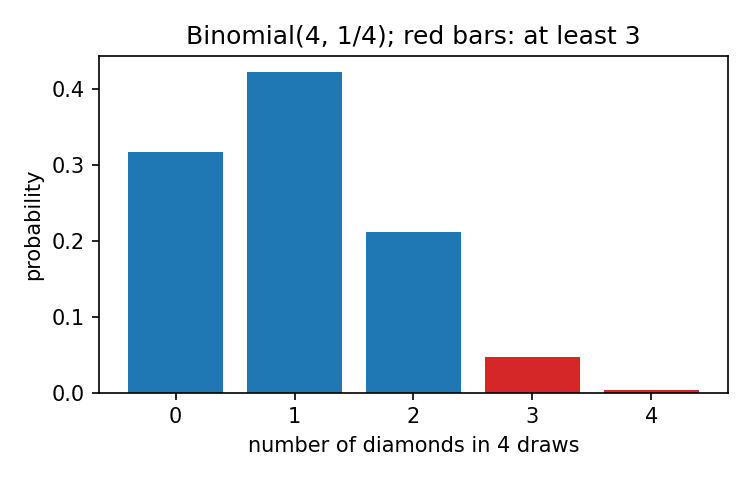
\includegraphics[width=0.55\linewidth]{figs/Cards.png}
    \caption{Distribution of the number of diamonds in four draws}
    \label{fig:cards_q6}
\end{figure}

    \item Find the value of $(x-y)$ from the matrix equation
\begin{align*}
    2\begin{bmatrix} x & 5 \\ 7 & y-3 \end{bmatrix} + \begin{bmatrix} -3 & -4 \\ 1 & 2 \end{bmatrix} = \begin{bmatrix} 7 & 6 \\ 15 & 14 \end{bmatrix}.
\end{align*}

\solution Moving the constant matrix to the right and dividing by $2$,
\begin{align}
    2\begin{bmatrix} x & 5 \\ 7 & y-3 \end{bmatrix} &= \begin{bmatrix} 7 & 6 \\ 15 & 14 \end{bmatrix} - \begin{bmatrix} -3 & -4 \\ 1 & 2 \end{bmatrix} = \begin{bmatrix} 10 & 10 \\ 14 & 12 \end{bmatrix} \\
    \begin{bmatrix} x & 5 \\ 7 & y-3 \end{bmatrix} &= \begin{bmatrix} 5 & 5 \\ 7 & 6 \end{bmatrix}
\end{align}
Comparing entries, $x = 5$ and $y - 3 = 6 \implies y = 9$. Hence
\begin{align}
    x - y = 5 - 9 = -4
\end{align}

    \item Solve the following differential equation:
\begin{align*}
    (y + 3x^2)\frac{dx}{dy} = x
\end{align*}

\solution Taking reciprocals, $\frac{dy}{dx} = \frac{y+3x^2}{x}$, which is linear in $y$:
\begin{align}
    \frac{dy}{dx} - \frac{1}{x}y = 3x
\end{align}
Here $P(x) = -\frac{1}{x}$, $Q(x) = 3x$. From \eqref{eq:EE26BTECH11225-linode},
\begin{align}
    \text{I.F.} &= e^{\int -\frac{1}{x}dx} = e^{-\ln x} = \frac{1}{x} \\
    \frac{y}{x} &= \int 3x\cdot\frac{1}{x}\,dx = 3x + C \\
    &\implies y = 3x^2 + Cx
\end{align}
The following code verifies the solution and plots \figref{fig:linearode_q8}.
\begin{lstlisting}[frame=single, basicstyle=\rmfamily, escapeinside={(*@}{@*)}]
(*@\makebox[\dimexpr\linewidth-2\fboxsep-2\fboxrule\relax][c]{codes/LinearOde.py}@*)
\end{lstlisting}
\begin{figure}[H]
    \centering
    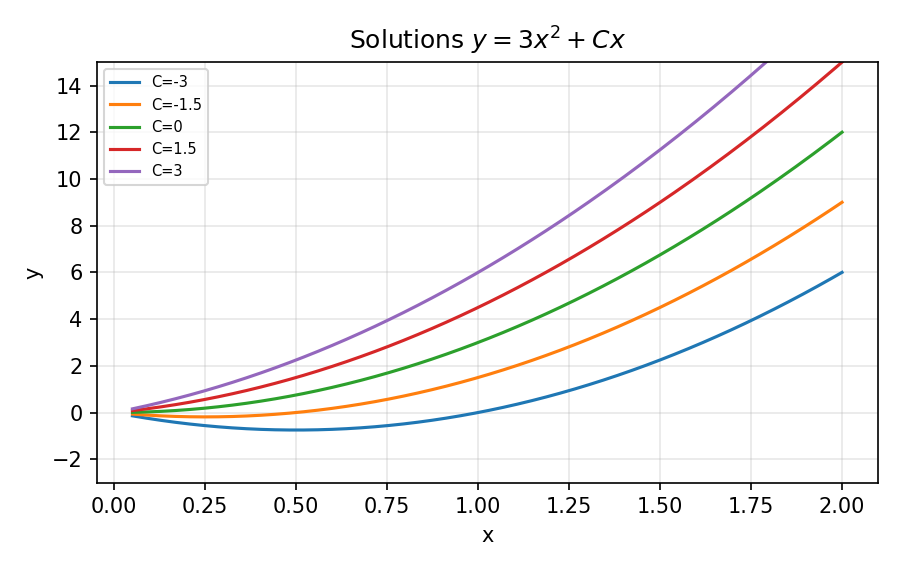
\includegraphics[width=0.70\linewidth]{figs/LinearOde.png}
    \caption{Solutions $y=3x^2+Cx$ for several values of $C$}
    \label{fig:linearode_q8}
\end{figure}

    \item
    \begin{enumerate}[label=(\alph*), leftmargin=1.5em, labelsep=0.5em]
        \item Using vectors, prove that the points $(2,-1,3)$, $(3,-5,1)$ and $(-1,11,9)$ are collinear.

        \begin{center}
            \textbf{OR}
        \end{center}

        \item For any two vectors $\vec{a}$ and $\vec{b}$, prove that $(\vec{a}\times\vec{b})^2 = \vec{a}^2\vec{b}^2 - (\vec{a}\cdot\vec{b})^2$.
    \end{enumerate} \vspace{2pt}
    \textbf{(a) Solution:} Let $A(2,-1,3)$, $B(3,-5,1)$, $C(-1,11,9)$.
\begin{align}
    \vec{AB} &= \myvec{3-2 \\ -5+1 \\ 1-3} = \myvec{1 \\ -4 \\ -2} \\
    \vec{BC} &= \myvec{-1-3 \\ 11+5 \\ 9-1} = \myvec{-4 \\ 16 \\ 8} = -4\myvec{1 \\ -4 \\ -2} = -4\,\vec{AB}
\end{align}
Since $\vec{BC} = k\,\vec{AB}$ with $k=-4$ and $B$ is common to both, the points $A$, $B$, $C$ are collinear. \\[8pt]
\textbf{(b) Solution:} Let $\theta$ be the angle between $\vec{a}$ and $\vec{b}$. From \eqref{eq:EE26BTECH11225-cross},
\begin{align}
    \|\vec{a}\times\vec{b}\|^2 &= \|\vec{a}\|^2\|\vec{b}\|^2\sin^2\theta \\
    &= \|\vec{a}\|^2\|\vec{b}\|^2\left(1-\cos^2\theta\right) \\
    &= \|\vec{a}\|^2\|\vec{b}\|^2 - \left(\|\vec{a}\|\|\vec{b}\|\cos\theta\right)^2
\end{align}
and, from \eqref{eq:EE26BTECH11225-dot}, $\|\vec{a}\|\|\vec{b}\|\cos\theta = \vec{a}^{\top}\vec{b}$. Hence
\begin{align}
    \|\vec{a}\times\vec{b}\|^2 = \|\vec{a}\|^2\|\vec{b}\|^2 - \left(\vec{a}^{\top}\vec{b}\right)^2
\end{align}
The following code verifies both parts and generates \figref{fig:collinear_q9}.
\begin{lstlisting}[frame=single, basicstyle=\rmfamily, escapeinside={(*@}{@*)}]
(*@\makebox[\dimexpr\linewidth-2\fboxsep-2\fboxrule\relax][c]{codes/Collinear.py}@*)
\end{lstlisting}
\begin{figure}[H]
    \centering
    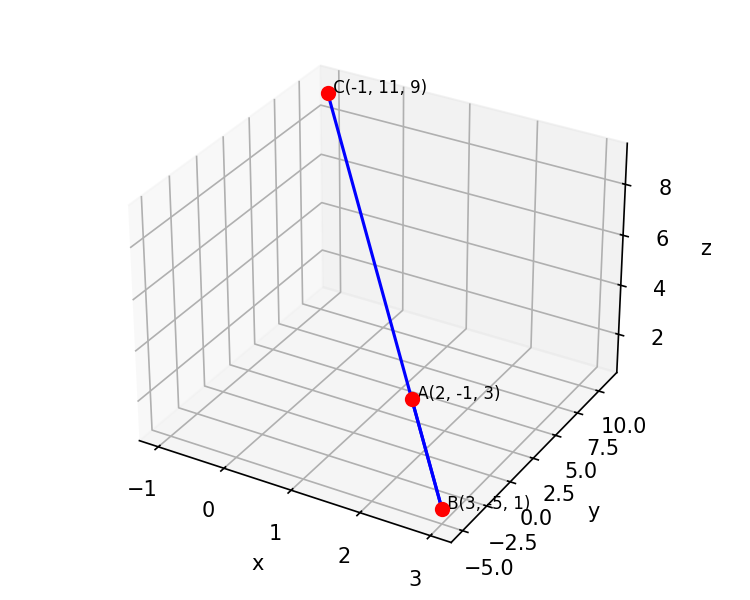
\includegraphics[width=0.55\linewidth]{figs/Collinear.png}
    \caption{The collinear points $A$, $B$, $C$}
    \label{fig:collinear_q9}
\end{figure}

    \item
    \begin{enumerate}[label=(\alph*), leftmargin=1.5em, labelsep=0.5em]
        \item Find: $\displaystyle\int\frac{x-1}{(x-2)(x-3)}\,dx$

        \begin{center}
            \textbf{OR}
        \end{center}

        \item Integrate: $\dfrac{e^x}{\sqrt{5-4e^x-e^{2x}}}$ with respect to $x$.
    \end{enumerate} \vspace{2pt}
    \textbf{(a) Solution:} Using partial fractions, $\frac{x-1}{(x-2)(x-3)} = \frac{A}{x-2}+\frac{B}{x-3}$:
\begin{align}
    A = \frac{2-1}{2-3} = -1, \quad B = \frac{3-1}{3-2} = 2
\end{align}
\begin{align}
    \int\frac{x-1}{(x-2)(x-3)}dx &= -\int\frac{dx}{x-2} + 2\int\frac{dx}{x-3} \\
    &= -\ln|x-2| + 2\ln|x-3| + C
\end{align}
\textbf{(b) Solution:} Let $t = e^x$, so $dt = e^x dx$. Since $5-4t-t^2 = 9-(t+2)^2$, from \eqref{eq:EE26BTECH11225-sininv}:
\begin{align}
    \int\frac{dt}{\sqrt{5-4t-t^2}} &= \int\frac{dt}{\sqrt{9-(t+2)^2}} \\
    &= \sin^{-1}\left(\frac{t+2}{3}\right) + C = \sin^{-1}\left(\frac{e^x+2}{3}\right) + C
\end{align}
(The integrand is real only for $e^x<1$, i.e. $x<0$.) The following code verifies both antiderivatives by differentiation.
\begin{lstlisting}[frame=single, basicstyle=\rmfamily, escapeinside={(*@}{@*)}]
(*@\makebox[\dimexpr\linewidth-2\fboxsep-2\fboxrule\relax][c]{codes/Partial.py}@*)
\end{lstlisting}

    \item Find: $\displaystyle\int e^x\left(\frac{2+\sin 2x}{2\cos^2 x}\right)dx$

\solution Using $\sin 2x = 2\sin x\cos x$:
\begin{align}
    \frac{2+\sin 2x}{2\cos^2 x} = \frac{1}{\cos^2 x} + \frac{2\sin x\cos x}{2\cos^2 x} = \sec^2 x + \tan x
\end{align}
With $f(x) = \tan x$ and $f'(x) = \sec^2 x$, from \eqref{eq:EE26BTECH11225-expint}:
\begin{align}
    \int e^x(\tan x+\sec^2 x)\,dx = e^x\tan x + C
\end{align}
The following code verifies the result by differentiation.
\begin{lstlisting}[frame=single, basicstyle=\rmfamily, escapeinside={(*@}{@*)}]
(*@\makebox[\dimexpr\linewidth-2\fboxsep-2\fboxrule\relax][c]{codes/ExpInt.py}@*)
\end{lstlisting}

    \item If $A$ and $B$ are independent events with $P(A) = \frac{3}{7}$ and $P(B) = \frac{2}{5}$, then find $P(A'\cap B')$.

\solution From \eqref{eq:EE26BTECH11225-indep-comp}:
\begin{align}
    P(A'\cap B') &= \left(1-\frac{3}{7}\right)\left(1-\frac{2}{5}\right) \\
    &= \frac{4}{7}\cdot\frac{3}{5} = \frac{12}{35}
\end{align}

    \item Find the equation of the plane passing through the point $(-1,3,2)$ and perpendicular to the planes $x+2y+3z=5$ and $3x+3y+z=0$.

\solution The normals of the given planes are $\vec{n}_1 = \myvec{1\\2\\3}$ and $\vec{n}_2 = \myvec{3\\3\\1}$. From \eqref{eq:EE26BTECH11225-plane},
\begin{align}
    \vec{n} = \vec{n}_1\times\vec{n}_2 = \myvec{2\cdot1-3\cdot3 \\ 3\cdot3-1\cdot1 \\ 1\cdot3-2\cdot3} = \myvec{-7 \\ 8 \\ -3}
\end{align}
The plane through $\vec{P}_0 = \myvec{-1\\3\\2}$ is $\vec{n}^{\top}(\vec{x}-\vec{P}_0) = 0$:
\begin{align}
    -7(x+1) + 8(y-3) - 3(z-2) &= 0 \\
    \implies -7x + 8y - 3z - 25 &= 0 \\
    \implies 7x - 8y + 3z + 25 &= 0
\end{align}
The following code verifies $\vec{n}\perp\vec{n}_1,\vec{n}_2$ and plots \figref{fig:plane_q13}.
\begin{lstlisting}[frame=single, basicstyle=\rmfamily, escapeinside={(*@}{@*)}]
(*@\makebox[\dimexpr\linewidth-2\fboxsep-2\fboxrule\relax][c]{codes/Plane13.py}@*)
\end{lstlisting}
\begin{figure}[H]
    \centering
    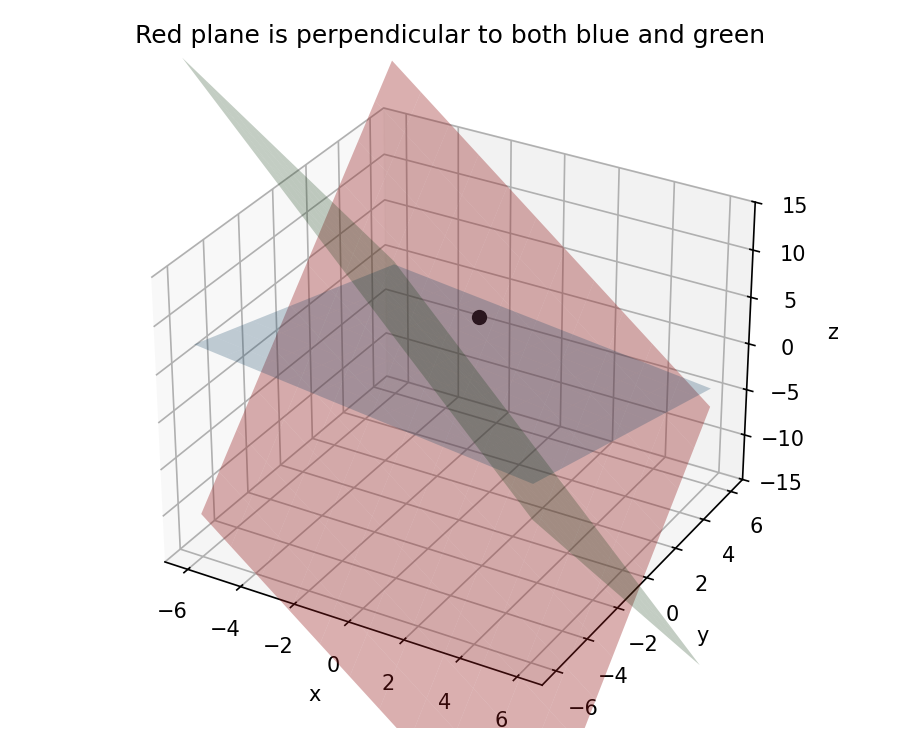
\includegraphics[width=0.65\linewidth]{figs/Plane13.png}
    \caption{The required plane (red) with the two given planes}
    \label{fig:plane_q13}
\end{figure}

    \item Evaluate: $\displaystyle\int_1^5 \big(|x-1| + |x-2| + |x-4|\big)\,dx$

\solution Using \eqref{eq:EE26BTECH11225-absint} for each term:
\begin{align}
    \int_1^5 |x-1|\,dx &= \int_1^5 (x-1)\,dx = \left[\frac{(x-1)^2}{2}\right]_1^5 = 8 \\
    \int_1^5 |x-2|\,dx &= \int_1^2 (2-x)\,dx + \int_2^5 (x-2)\,dx = \frac{1}{2}+\frac{9}{2} = 5 \\
    \int_1^5 |x-4|\,dx &= \int_1^4 (4-x)\,dx + \int_4^5 (x-4)\,dx = \frac{9}{2}+\frac{1}{2} = 5
\end{align}
Adding,
\begin{align}
    \int_1^5 \big(|x-1|+|x-2|+|x-4|\big)dx = 8+5+5 = 18
\end{align}
The following code verifies the value and plots \figref{fig:absint_q14}.
\begin{lstlisting}[frame=single, basicstyle=\rmfamily, escapeinside={(*@}{@*)}]
(*@\makebox[\dimexpr\linewidth-2\fboxsep-2\fboxrule\relax][c]{codes/AbsInt.py}@*)
\end{lstlisting}
\begin{figure}[H]
    \centering
    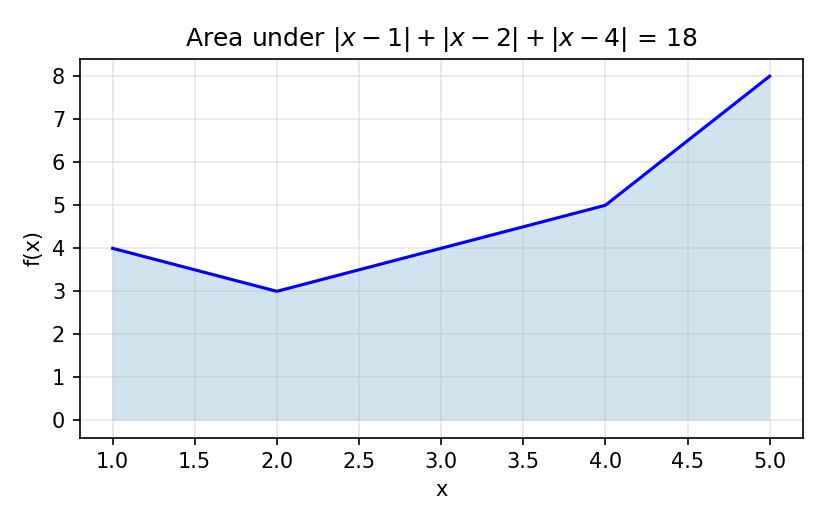
\includegraphics[width=0.60\linewidth]{figs/AbsInt.png}
    \caption{Area under $|x-1|+|x-2|+|x-4|$ from $x=1$ to $x=5$}
    \label{fig:absint_q14}
\end{figure}

    \item If $x,y,z$ are different and $\Delta = \begin{vmatrix} x & x^2 & x^3-1 \\ y & y^2 & y^3-1 \\ z & z^2 & z^3-1 \end{vmatrix} = 0$, then using properties of determinants, show that $xyz=1$.

\solution Splitting the third column:
\begin{align}
    \Delta &= \begin{vmatrix} x & x^2 & x^3 \\ y & y^2 & y^3 \\ z & z^2 & z^3 \end{vmatrix} - \begin{vmatrix} x & x^2 & 1 \\ y & y^2 & 1 \\ z & z^2 & 1 \end{vmatrix}
\end{align}
Taking $x$, $y$, $z$ common from the rows of the first determinant, and moving the last column of the second determinant to the front (two column interchanges, so the sign is unchanged):
\begin{align}
    \Delta &= xyz\begin{vmatrix} 1 & x & x^2 \\ 1 & y & y^2 \\ 1 & z & z^2 \end{vmatrix} - \begin{vmatrix} 1 & x & x^2 \\ 1 & y & y^2 \\ 1 & z & z^2 \end{vmatrix} \\
    &= (xyz-1)\begin{vmatrix} 1 & x & x^2 \\ 1 & y & y^2 \\ 1 & z & z^2 \end{vmatrix} \\
    &= (xyz-1)(y-x)(z-x)(z-y) = 0
\end{align}
Since $x,y,z$ are different, $(y-x)(z-x)(z-y)\neq 0$. Hence $xyz - 1 = 0$, i.e. $xyz = 1$. The following code factorises $\Delta$ symbolically.
\begin{lstlisting}[frame=single, basicstyle=\rmfamily, escapeinside={(*@}{@*)}]
(*@\makebox[\dimexpr\linewidth-2\fboxsep-2\fboxrule\relax][c]{codes/Det3.py}@*)
\end{lstlisting}

    \item Prove that: $\sin^{-1}\dfrac{4}{5} + \tan^{-1}\dfrac{5}{12} + \cos^{-1}\dfrac{63}{65} = \dfrac{\pi}{2}$

\solution Write $\sin^{-1}\frac{4}{5}$ and $\cos^{-1}\frac{63}{65}$ in terms of $\tan^{-1}$ (from the right triangles with sides $3,4,5$ and $16,63,65$):
\begin{align}
    \sin^{-1}\frac{4}{5} = \tan^{-1}\frac{4}{3}, \quad \cos^{-1}\frac{63}{65} = \tan^{-1}\frac{16}{63}
\end{align}
From \eqref{eq:EE26BTECH11225-invtrig-2} (here $ab = \frac{4}{3}\cdot\frac{5}{12} = \frac{5}{9} < 1$):
\begin{align}
    \tan^{-1}\frac{4}{3}+\tan^{-1}\frac{5}{12} &= \tan^{-1}\frac{\frac{4}{3}+\frac{5}{12}}{1-\frac{20}{36}} = \tan^{-1}\frac{63}{16}
\end{align}
Since $\tan^{-1}\frac{16}{63} = \cot^{-1}\frac{63}{16}$, from \eqref{eq:EE26BTECH11225-invtrig-3}:
\begin{align}
    \text{LHS} = \tan^{-1}\frac{63}{16}+\cot^{-1}\frac{63}{16} = \frac{\pi}{2} = \text{RHS}
\end{align}
Hence proved. The following code verifies each step numerically.
\begin{lstlisting}[frame=single, basicstyle=\rmfamily, escapeinside={(*@}{@*)}]
(*@\makebox[\dimexpr\linewidth-2\fboxsep-2\fboxrule\relax][c]{codes/InvSum.py}@*)
\end{lstlisting}

    \item Using vectors, find the value of $x$ such that the four points $A(x,5,-1)$, $B(3,2,1)$, $C(4,5,5)$ and $D(4,2,-2)$ are coplanar.

\solution From \eqref{eq:EE26BTECH11225-coplanar}, the points are coplanar if $\det\begin{bmatrix}\vec{AB} & \vec{AC} & \vec{AD}\end{bmatrix}=0$. Here
\begin{align}
    \vec{AB} = \myvec{3-x \\ -3 \\ 2}, \quad \vec{AC} = \myvec{4-x \\ 0 \\ 6}, \quad \vec{AD} = \myvec{4-x \\ -3 \\ -1}
\end{align}
\begin{align}
    \begin{vmatrix} 3-x & 4-x & 4-x \\ -3 & 0 & -3 \\ 2 & 6 & -1 \end{vmatrix} &= 0 \\
    (3-x)\big[0+18\big] - (4-x)\big[3+6\big] + (4-x)\big[-18-0\big] &= 0 \\
    18(3-x) - 9(4-x) - 18(4-x) &= 0 \\
    54 - 18x - 27(4-x) &= 0 \\
    9x - 54 &= 0 \implies x = 6
\end{align}
The following code solves for $x$, checks that the determinant vanishes at $x=6$ and plots \figref{fig:coplanar_q17}.
\begin{lstlisting}[frame=single, basicstyle=\rmfamily, escapeinside={(*@}{@*)}]
(*@\makebox[\dimexpr\linewidth-2\fboxsep-2\fboxrule\relax][c]{codes/Coplanar.py}@*)
\end{lstlisting}
\begin{figure}[H]
    \centering
    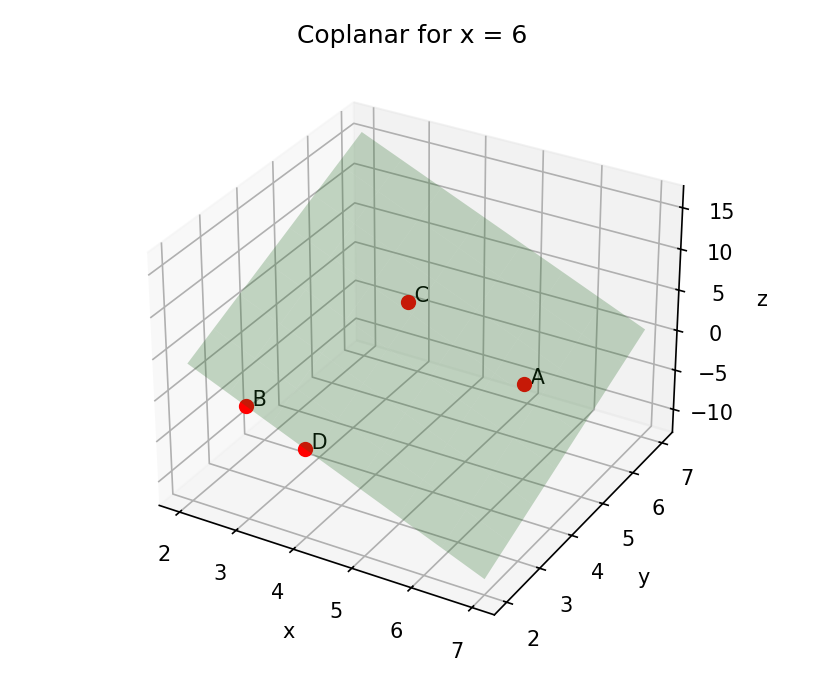
\includegraphics[width=0.60\linewidth]{figs/Coplanar.png}
    \caption{The four coplanar points for $x=6$}
    \label{fig:coplanar_q17}
\end{figure}

    \item
    \begin{enumerate}[label=(\alph*), leftmargin=1.5em, labelsep=0.5em]
        \item Differentiate $\tan^{-1}\dfrac{3x-x^3}{1-3x^2}$, $|x|<\dfrac{1}{\sqrt{3}}$ w.r.t. $\tan^{-1}\dfrac{x}{\sqrt{1-x^2}}$.

        \begin{center}
            \textbf{OR}
        \end{center}

        \item If $\sqrt{1-x^2}+\sqrt{1-y^2} = a(x-y)$, $|x|<1$, $|y|<1$, show that $\dfrac{dy}{dx} = \sqrt{\dfrac{1-y^2}{1-x^2}}$.
    \end{enumerate} \vspace{2pt}
    \textbf{(a) Solution:} Let $u = \tan^{-1}\frac{3x-x^3}{1-3x^2}$ and $v = \tan^{-1}\frac{x}{\sqrt{1-x^2}}$. Put $x=\tan\phi$; since $|x|<\frac{1}{\sqrt{3}}$, $|3\phi|<\frac{\pi}{2}$ and
\begin{align}
    u = \tan^{-1}(\tan 3\phi) = 3\phi = 3\tan^{-1}x \implies \frac{du}{dx} = \frac{3}{1+x^2}
\end{align}
From \eqref{eq:EE26BTECH11225-invtrig-4}, $v = \sin^{-1}x$, so $\frac{dv}{dx} = \frac{1}{\sqrt{1-x^2}}$. Hence
\begin{align}
    \frac{du}{dv} = \frac{du/dx}{dv/dx} = \frac{3\sqrt{1-x^2}}{1+x^2}
\end{align}
\textbf{(b) Solution:} Put $x=\sin\alpha$, $y=\sin\beta$ with $\alpha,\beta\in\left(-\frac{\pi}{2},\frac{\pi}{2}\right)$:
\begin{align}
    \cos\alpha + \cos\beta &= a(\sin\alpha - \sin\beta) \\
    2\cos\frac{\alpha+\beta}{2}\cos\frac{\alpha-\beta}{2} &= 2a\cos\frac{\alpha+\beta}{2}\sin\frac{\alpha-\beta}{2} \\
    \implies \cot\frac{\alpha-\beta}{2} = a &\implies \sin^{-1}x - \sin^{-1}y = 2\cot^{-1}a
\end{align}
Differentiating w.r.t. $x$ (the right side is a constant):
\begin{align}
    \frac{1}{\sqrt{1-x^2}} - \frac{1}{\sqrt{1-y^2}}\frac{dy}{dx} = 0 \implies \frac{dy}{dx} = \sqrt{\frac{1-y^2}{1-x^2}}
\end{align}
The following code verifies both parts and plots \figref{fig:diff_q18}.
\begin{lstlisting}[frame=single, basicstyle=\rmfamily, escapeinside={(*@}{@*)}]
(*@\makebox[\dimexpr\linewidth-2\fboxsep-2\fboxrule\relax][c]{codes/Differentiate.py}@*)
\end{lstlisting}
\begin{figure}[H]
    \centering
    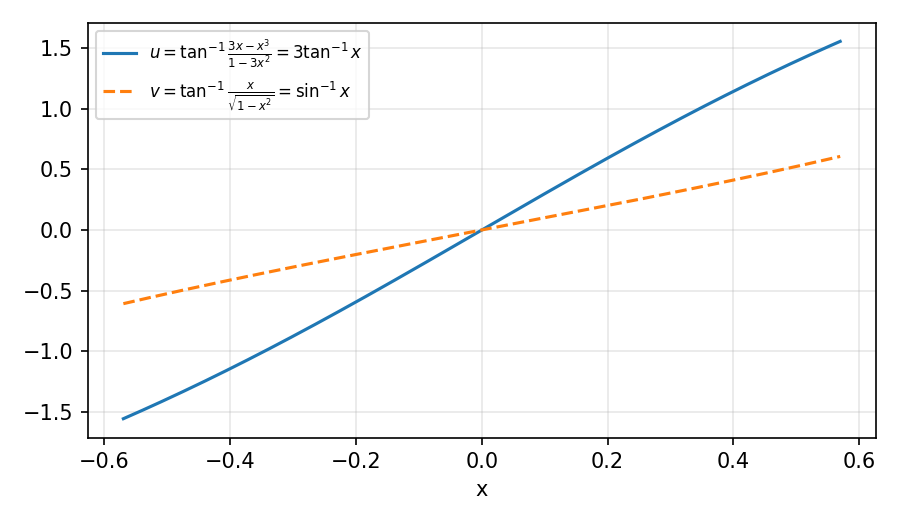
\includegraphics[width=0.65\linewidth]{figs/Differentiate.png}
    \caption{The functions $u=3\tan^{-1}x$ and $v=\sin^{-1}x$}
    \label{fig:diff_q18}
\end{figure}

    \item
    \begin{enumerate}[label=(\alph*), leftmargin=1.5em, labelsep=0.5em]
        \item Prove that the relation $R$ in the set $A = \{1,2,3,4,5,6,7\}$ given by $R = \{(a,b) : |a-b| \text{ is even}\}$ is an equivalence relation.

        \begin{center}
            \textbf{OR}
        \end{center}

        \item Show that the function $f$ in $A = \mathbb{R}-\left\{\frac{2}{3}\right\}$ defined as $f(x) = \dfrac{4x+3}{6x-4}$ is one-one and onto. Hence, find $f^{-1}$.
    \end{enumerate} \vspace{2pt}
    \textbf{(a) Solution:} By \ref{eq:EE26BTECH11225-equiv} we check three properties.
\begin{align}
    \text{Reflexive: } & |a-a| = 0 \text{ is even} \implies (a,a)\in R \\
    \text{Symmetric: } & |a-b| = |b-a| \implies (a,b)\in R \Rightarrow (b,a)\in R \\
    \text{Transitive: } & |a-b|,\,|b-c| \text{ even} \implies a-c = (a-b)+(b-c) \text{ is even}
\end{align}
Hence $R$ is an equivalence relation. \\[8pt]
\textbf{(b) Solution:} \emph{One-one:} Let $f(x_1) = f(x_2)$:
\begin{align}
    (4x_1+3)(6x_2-4) &= (4x_2+3)(6x_1-4) \\
    24x_1x_2 - 16x_1 + 18x_2 - 12 &= 24x_1x_2 - 16x_2 + 18x_1 - 12 \\
    34x_2 = 34x_1 &\implies x_1 = x_2
\end{align}
\emph{Onto:} Let $y = \frac{4x+3}{6x-4}$, $y \neq \frac{2}{3}$. Solving for $x$:
\begin{align}
    6xy - 4y = 4x+3 \implies x = \frac{4y+3}{6y-4}
\end{align}
This $x$ is defined for every $y\neq\frac{2}{3}$, and $x\neq\frac{2}{3}$ (otherwise $12y+9=12y-8$, which is impossible). So every $y\in A$ has a pre-image and $f$ is onto. Hence
\begin{align}
    f^{-1}(y) = \frac{4y+3}{6y-4}, \quad \text{i.e. } f^{-1} = f
\end{align}
The following code verifies both parts and generates \figref{fig:equiv_q19}.
\begin{lstlisting}[frame=single, basicstyle=\rmfamily, escapeinside={(*@}{@*)}]
(*@\makebox[\dimexpr\linewidth-2\fboxsep-2\fboxrule\relax][c]{codes/Equiv.py}@*)
\end{lstlisting}
\begin{figure}[H]
    \centering
    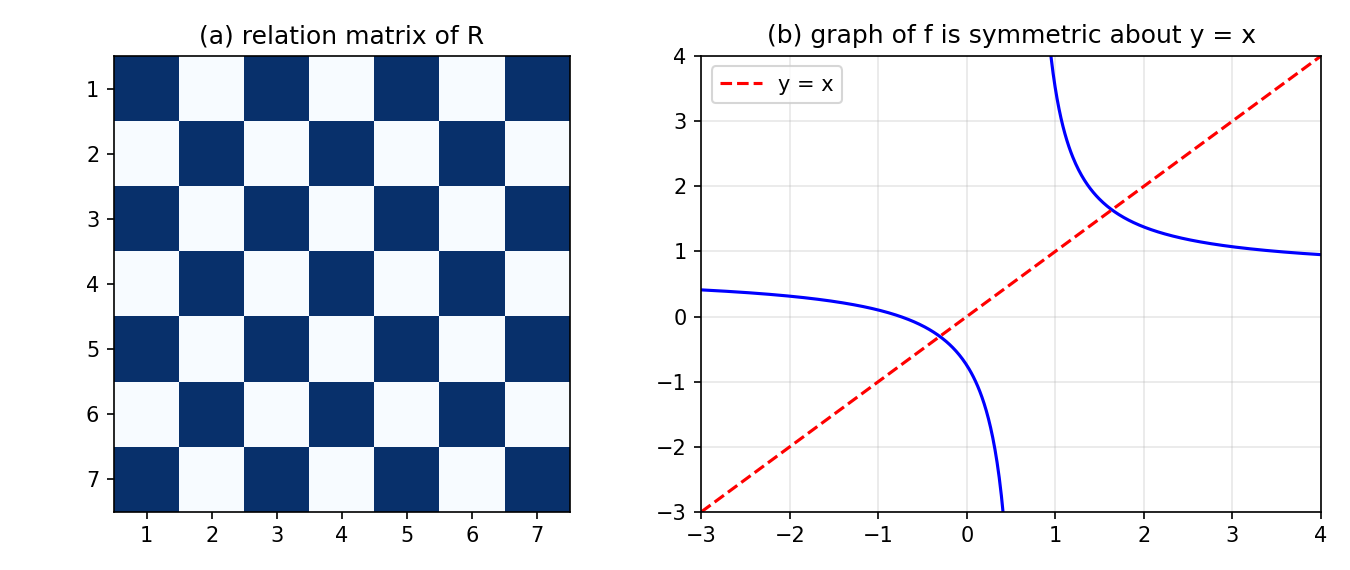
\includegraphics[width=0.95\linewidth]{figs/Equiv.png}
    \caption{(a) Relation matrix of $R$; (b) graph of $f$, symmetric about $y=x$}
    \label{fig:equiv_q19}
\end{figure}

    \item
    \begin{enumerate}[label=(\alph*), leftmargin=1.5em, labelsep=0.5em]
        \item Find the particular solution of the differential equation $(1+e^{2x})\,dy + (1+y^2)e^x\,dx = 0$, given that $y(0)=1$.

        \begin{center}
            \textbf{OR}
        \end{center}

        \item Find the particular solution of the differential equation $x\dfrac{dy}{dx}\sin\left(\dfrac{y}{x}\right) + x - y\sin\left(\dfrac{y}{x}\right) = 0$, given that $y(1) = \dfrac{\pi}{2}$.
    \end{enumerate} \vspace{2pt}
    \textbf{(a) Solution:} Separating the variables:
\begin{align}
    \frac{dy}{1+y^2} &= -\frac{e^x\,dx}{1+e^{2x}} \\
    \tan^{-1}y &= -\tan^{-1}(e^x) + C
\end{align}
Using $y(0)=1$: $\frac{\pi}{4} = -\frac{\pi}{4}+C \implies C = \frac{\pi}{2}$. Then from \eqref{eq:EE26BTECH11225-invtrig-3},
\begin{align}
    \tan^{-1}y = \frac{\pi}{2}-\tan^{-1}(e^x) = \cot^{-1}(e^x) = \tan^{-1}(e^{-x}) \implies y = e^{-x}
\end{align}
\textbf{(b) Solution:} Dividing by $x\sin\left(\frac{y}{x}\right)$:
\begin{align}
    \frac{dy}{dx} = \frac{y}{x} - \frac{1}{\sin(y/x)}
\end{align}
This is homogeneous. From \eqref{eq:EE26BTECH11225-homog}, put $y=vx$:
\begin{align}
    v + x\frac{dv}{dx} &= v - \frac{1}{\sin v} \\
    \sin v\,dv &= -\frac{dx}{x} \\
    -\cos v &= -\ln|x| + C \implies \cos\left(\frac{y}{x}\right) = \ln|x| + C'
\end{align}
Using $y(1)=\frac{\pi}{2}$: $\cos\frac{\pi}{2} = 0 = \ln 1 + C' \implies C'=0$. Hence
\begin{align}
    \cos\left(\frac{y}{x}\right) = \ln|x|
\end{align}
The following code verifies both solutions and plots \figref{fig:solveode_q20}.
\begin{lstlisting}[frame=single, basicstyle=\rmfamily, escapeinside={(*@}{@*)}]
(*@\makebox[\dimexpr\linewidth-2\fboxsep-2\fboxrule\relax][c]{codes/SolveOde.py}@*)
\end{lstlisting}
\begin{figure}[H]
    \centering
    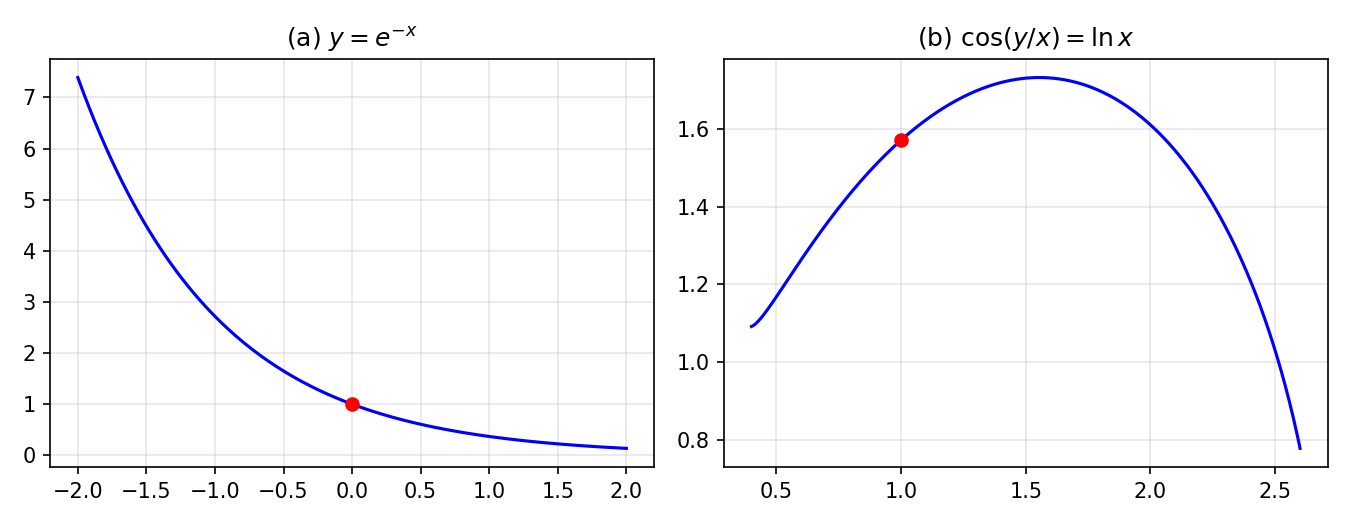
\includegraphics[width=0.95\linewidth]{figs/SolveOde.png}
    \caption{(a) $y=e^{-x}$ and (b) $\cos(y/x)=\ln x$}
    \label{fig:solveode_q20}
\end{figure}

    \item If $y = (\sin x)^x + \sin^{-1}\left(\sqrt{1-x^2}\right)$, then find $\dfrac{dy}{dx}$.

\solution The function is defined for $0<x<1$ (we need $\sin x>0$ and $|x|\leq1$). Let $y = u + w$ with $u = (\sin x)^x$ and $w = \sin^{-1}\sqrt{1-x^2}$. From \eqref{eq:EE26BTECH11225-logdiff}:
\begin{align}
    \ln u = x\ln\sin x &\implies \frac{1}{u}\frac{du}{dx} = \ln\sin x + x\cot x \\
    &\implies \frac{du}{dx} = (\sin x)^x\left(x\cot x + \ln\sin x\right)
\end{align}
For $0<x<1$ put $x=\cos\phi$, $\phi\in\left(0,\frac{\pi}{2}\right)$; then $\sqrt{1-x^2}=\sin\phi$ and $w = \phi = \cos^{-1}x$:
\begin{align}
    \frac{dw}{dx} = -\frac{1}{\sqrt{1-x^2}}
\end{align}
Hence
\begin{align}
    \frac{dy}{dx} = (\sin x)^x\left(x\cot x+\ln\sin x\right) - \frac{1}{\sqrt{1-x^2}}
\end{align}
The following code verifies the derivative and plots \figref{fig:logdiff_q21}.
\begin{lstlisting}[frame=single, basicstyle=\rmfamily, escapeinside={(*@}{@*)}]
(*@\makebox[\dimexpr\linewidth-2\fboxsep-2\fboxrule\relax][c]{codes/LogDiff.py}@*)
\end{lstlisting}
\begin{figure}[H]
    \centering
    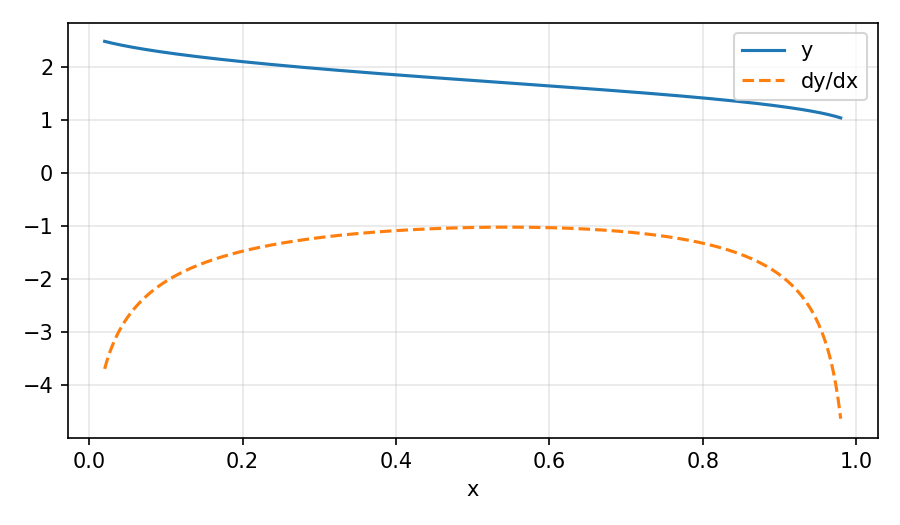
\includegraphics[width=0.65\linewidth]{figs/LogDiff.png}
    \caption{The function $y$ and its derivative on $(0,1)$}
    \label{fig:logdiff_q21}
\end{figure}

    \item Find: $\displaystyle\int\cos 2x\cos 4x\cos 6x\,dx$

\solution From \eqref{eq:EE26BTECH11225-prodsum}, $\cos 2x\cos 4x = \frac{1}{2}(\cos 6x+\cos 2x)$:
\begin{align}
    \cos 2x\cos 4x\cos 6x &= \frac{1}{2}\left(\cos^2 6x + \cos 2x\cos 6x\right) \\
    &= \frac{1}{2}\left(\frac{1+\cos 12x}{2}+\frac{\cos 8x+\cos 4x}{2}\right) \\
    &= \frac{1}{4}\left(1+\cos 12x+\cos 8x+\cos 4x\right)
\end{align}
Integrating,
\begin{align}
    \int\cos 2x\cos 4x\cos 6x\,dx = \frac{1}{4}\left[x+\frac{\sin 12x}{12}+\frac{\sin 8x}{8}+\frac{\sin 4x}{4}\right] + C
\end{align}
The following code verifies the result by differentiation.
\begin{lstlisting}[frame=single, basicstyle=\rmfamily, escapeinside={(*@}{@*)}]
(*@\makebox[\dimexpr\linewidth-2\fboxsep-2\fboxrule\relax][c]{codes/CosProd.py}@*)
\end{lstlisting}

    \item Find the interval in which the function $f$ given by $f(x) = \sin 2x + \cos 2x$, $0\leq x\leq\pi$ is strictly decreasing.

\solution Differentiating,
\begin{align}
    f'(x) &= 2\cos 2x - 2\sin 2x = 2\sqrt{2}\cos\left(2x+\frac{\pi}{4}\right)
\end{align}
From \ref{eq:EE26BTECH11225-mono}, $f$ is strictly decreasing where $f'(x)<0$. For $0\leq x\leq\pi$, $2x+\frac{\pi}{4}\in\left[\frac{\pi}{4},\frac{9\pi}{4}\right]$, and $\cos\theta<0$ there only for $\frac{\pi}{2}<\theta<\frac{3\pi}{2}$:
\begin{align}
    \frac{\pi}{2} < 2x+\frac{\pi}{4} < \frac{3\pi}{2} \implies \frac{\pi}{8} < x < \frac{5\pi}{8}
\end{align}
Thus $f$ is strictly decreasing on $\left(\frac{\pi}{8},\frac{5\pi}{8}\right)$. The following code verifies the interval and plots \figref{fig:decreasing_q23}.
\begin{lstlisting}[frame=single, basicstyle=\rmfamily, escapeinside={(*@}{@*)}]
(*@\makebox[\dimexpr\linewidth-2\fboxsep-2\fboxrule\relax][c]{codes/Decreasing.py}@*)
\end{lstlisting}
\begin{figure}[H]
    \centering
    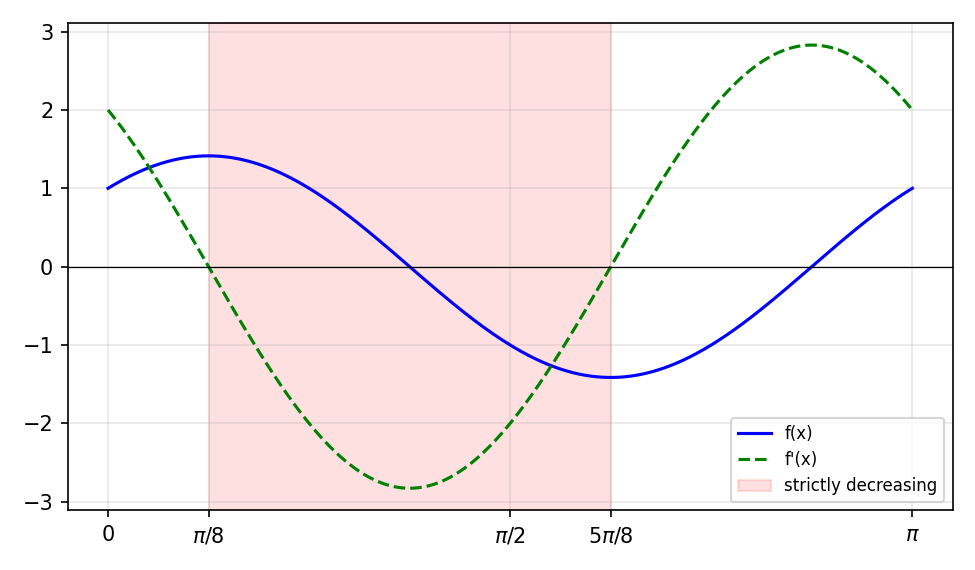
\includegraphics[width=0.70\linewidth]{figs/Decreasing.png}
    \caption{$f(x)=\sin 2x+\cos 2x$ and $f'(x)$}
    \label{fig:decreasing_q23}
\end{figure}

    \item
    \begin{enumerate}[label=(\alph*), leftmargin=1.5em, labelsep=0.5em]
        \item Using elementary row transformations, find the inverse of the matrix
        \begin{align*}
            \begin{bmatrix} 3 & 0 & -1 \\ 2 & 3 & 0 \\ 0 & 4 & 1 \end{bmatrix}
        \end{align*}

        \begin{center}
            \textbf{OR}
        \end{center}

        \item Using matrices, solve the following system of linear equations:
        \begin{align*}
            2x+3y+10z &= 4 \\
            4x-6y+5z &= 1 \\
            6x+9y-20z &= 2
        \end{align*}
    \end{enumerate} \vspace{2pt}
    \textbf{(a) Solution:} From \eqref{eq:EE26BTECH11225-rowops}, apply row operations to $[A\,|\,I]$:
\begin{align}
    [A|I] &= \left[\begin{array}{ccc|ccc} 3 & 0 & -1 & 1 & 0 & 0 \\ 2 & 3 & 0 & 0 & 1 & 0 \\ 0 & 4 & 1 & 0 & 0 & 1 \end{array}\right] \\
    \xrightarrow{R_1\to R_1-R_2}\; &\left[\begin{array}{ccc|ccc} 1 & -3 & -1 & 1 & -1 & 0 \\ 2 & 3 & 0 & 0 & 1 & 0 \\ 0 & 4 & 1 & 0 & 0 & 1 \end{array}\right] \\
    \xrightarrow{R_2\to R_2-2R_1}\; &\left[\begin{array}{ccc|ccc} 1 & -3 & -1 & 1 & -1 & 0 \\ 0 & 9 & 2 & -2 & 3 & 0 \\ 0 & 4 & 1 & 0 & 0 & 1 \end{array}\right] \\
    \xrightarrow{R_2\to R_2-2R_3}\; &\left[\begin{array}{ccc|ccc} 1 & -3 & -1 & 1 & -1 & 0 \\ 0 & 1 & 0 & -2 & 3 & -2 \\ 0 & 4 & 1 & 0 & 0 & 1 \end{array}\right] \\
    \xrightarrow{R_1\to R_1+3R_2}\; &\left[\begin{array}{ccc|ccc} 1 & 0 & -1 & -5 & 8 & -6 \\ 0 & 1 & 0 & -2 & 3 & -2 \\ 0 & 4 & 1 & 0 & 0 & 1 \end{array}\right] \\
    \xrightarrow{R_3\to R_3-4R_2}\; &\left[\begin{array}{ccc|ccc} 1 & 0 & -1 & -5 & 8 & -6 \\ 0 & 1 & 0 & -2 & 3 & -2 \\ 0 & 0 & 1 & 8 & -12 & 9 \end{array}\right] \\
    \xrightarrow{R_1\to R_1+R_3}\; &\left[\begin{array}{ccc|ccc} 1 & 0 & 0 & 3 & -4 & 3 \\ 0 & 1 & 0 & -2 & 3 & -2 \\ 0 & 0 & 1 & 8 & -12 & 9 \end{array}\right]
\end{align}
Thus,
\begin{align}
    A^{-1} = \begin{bmatrix} 3 & -4 & 3 \\ -2 & 3 & -2 \\ 8 & -12 & 9 \end{bmatrix}
\end{align}
\textbf{(b) Solution:} Write the system as $A\vec{x}=\vec{b}$ and apply row operations to the augmented matrix $[A\,|\,\vec{b}]$, as in \eqref{eq:EE26BTECH11225-rowops}:
\begin{align}
    \big[A\,|\,\vec{b}\big] &= \left[\begin{array}{ccc|c} 2 & 3 & 10 & 4 \\ 4 & -6 & 5 & 1 \\ 6 & 9 & -20 & 2 \end{array}\right] \\
    \xrightarrow[R_3\to R_3-3R_1]{R_2\to R_2-2R_1}\; &\left[\begin{array}{ccc|c} 2 & 3 & 10 & 4 \\ 0 & -12 & -15 & -7 \\ 0 & 0 & -50 & -10 \end{array}\right]
\end{align}
These operations do not change the determinant, so $|A| = 2(-12)(-50) = 1200 \neq 0$ and the solution is unique (see \eqref{eq:EE26BTECH11225-adj}). By back-substitution,
\begin{align}
    -50z = -10 &\implies z = \frac{1}{5} \\
    -12y - 15\left(\frac{1}{5}\right) = -7 &\implies y = \frac{1}{3} \\
    2x + 3\left(\frac{1}{3}\right) + 10\left(\frac{1}{5}\right) = 4 &\implies x = \frac{1}{2}
\end{align}
Thus $x = \frac{1}{2}$, $y = \frac{1}{3}$, $z = \frac{1}{5}$. The following code carries out the row operations step by step and solves the system.
\begin{lstlisting}[frame=single, basicstyle=\rmfamily, escapeinside={(*@}{@*)}]
(*@\makebox[\dimexpr\linewidth-2\fboxsep-2\fboxrule\relax][c]{codes/Inverse.py}@*)
\end{lstlisting}

    \item
    \begin{enumerate}[label=(\alph*), leftmargin=1.5em, labelsep=0.5em]
        \item Using integration, find the area of the following region: $\{(x,y) : x^2+y^2\leq 16a^2 \text{ and } y^2\leq 6ax\}$

        \begin{center}
            \textbf{OR}
        \end{center}

        \item Using integration, find the area of triangle $ABC$ bounded by the lines $4x-y+5=0$, $x+y-5=0$ and $x-4y+5=0$.
    \end{enumerate} \vspace{2pt}
    \textbf{(a) Solution:} The circle $x^2+y^2=16a^2$ and the parabola $y^2=6ax$ meet where
\begin{align}
    x^2+6ax-16a^2 = 0 \implies (x+8a)(x-2a) = 0 \implies x = 2a, \quad y = \pm 2\sqrt{3}\,a
\end{align}
Writing both curves as $x$ in terms of $y$, the parabola $x = \frac{y^2}{6a}$ is the left boundary and the circle $x = \sqrt{16a^2-y^2}$ is the right boundary. The region is symmetric about the $x$-axis, so from \eqref{eq:EE26BTECH11225-area-curves-y},
\begin{align}
    \text{Area} &= 2\int_0^{2\sqrt{3}a}\left(\sqrt{16a^2-y^2}-\frac{y^2}{6a}\right)dy
\end{align}
From \eqref{eq:EE26BTECH11225-sqrtint},
\begin{align}
    &= 2\left[\frac{y}{2}\sqrt{16a^2-y^2}+8a^2\sin^{-1}\frac{y}{4a}-\frac{y^3}{18a}\right]_0^{2\sqrt{3}a} \\
    &= 2\left[2\sqrt{3}a^2+\frac{8\pi a^2}{3}-\frac{4\sqrt{3}a^2}{3}\right] \\
    &= \frac{4a^2}{3}\left(4\pi+\sqrt{3}\right)\text{ sq. units}
\end{align}
\textbf{(b) Solution:} Solving the lines pairwise gives the vertices $A(-1,1)$ (lines 1 and 3), $B(0,5)$ (lines 1 and 2) and $C(3,2)$ (lines 2 and 3). Between $x=-1$ and $x=0$ the upper boundary is $y=4x+5$, between $x=0$ and $x=3$ it is $y=5-x$, and the lower boundary is $y=\frac{x+5}{4}$. From \eqref{eq:EE26BTECH11225-area-curves},
\begin{align}
    \text{Area} &= \int_{-1}^{0}\left(4x+5-\frac{x+5}{4}\right)dx + \int_{0}^{3}\left(5-x-\frac{x+5}{4}\right)dx \\
    &= \frac{15}{4}\left[\frac{x^2}{2}+x\right]_{-1}^{0} + \left[\frac{15x}{4}-\frac{5x^2}{8}\right]_0^3 \\
    &= \frac{15}{8} + \frac{45}{8} = \frac{15}{2}\text{ sq. units}
\end{align}
This agrees with \eqref{eq:EE26BTECH11225-area-tri}. The following code verifies both parts and generates \figref{fig:area_q25}.
\begin{lstlisting}[frame=single, basicstyle=\rmfamily, escapeinside={(*@}{@*)}]
(*@\makebox[\dimexpr\linewidth-2\fboxsep-2\fboxrule\relax][c]{codes/Area.py}@*)
\end{lstlisting}
\begin{figure}[H]
    \centering
    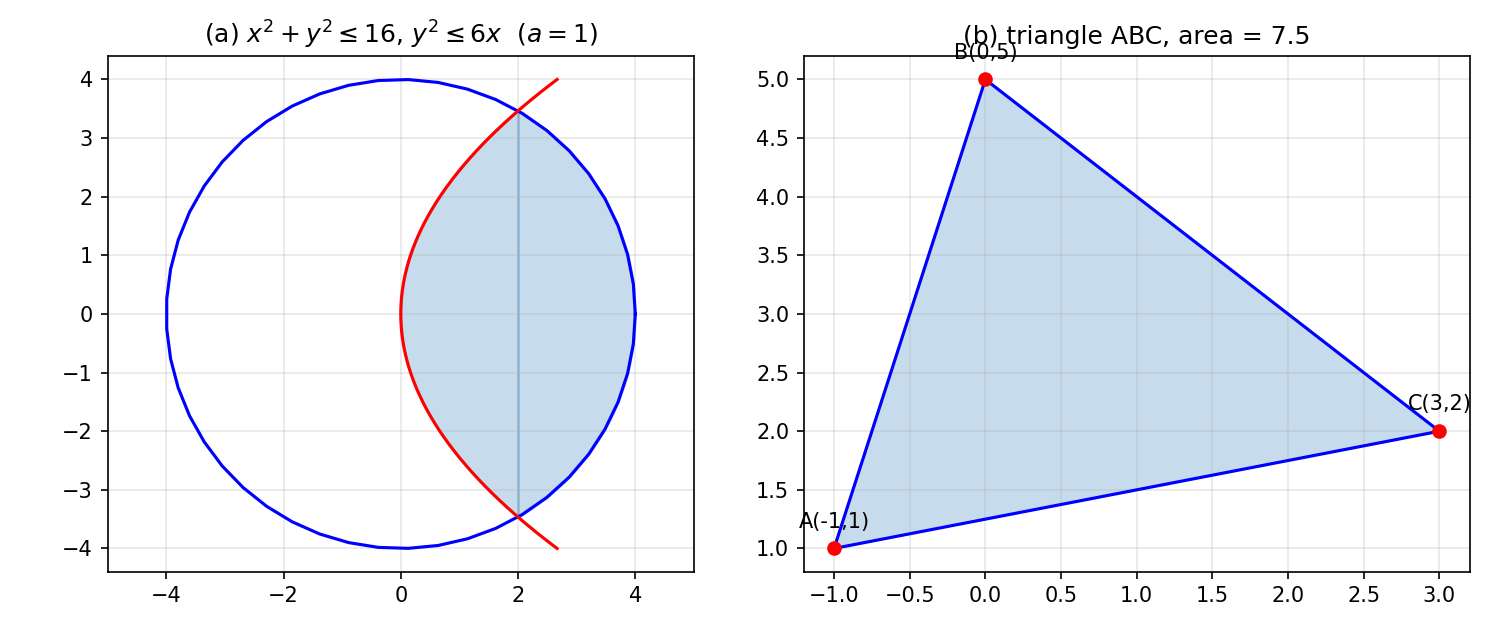
\includegraphics[width=0.95\linewidth]{figs/Area.png}
    \caption{(a) Region inside the circle and the parabola ($a=1$); (b) triangle $ABC$}
    \label{fig:area_q25}
\end{figure}

    \item A company manufactures two types of novelty souvenirs made of plywood. Souvenirs of type A require 5 minutes each for cutting and 10 minutes each for assembling. Souvenirs of type B require 8 minutes each for cutting and 8 minutes each for assembling. There are 3 hours 20 minutes available for cutting and 4 hours for assembling. The profit for type A souvenirs is \rupee 100 each and for type B souvenirs, profit is \rupee 120 each. How many souvenirs of each type should the company manufacture in order to maximise the profit? Formulate the problem as a LPP and then solve it graphically.

\solution Let the company make $x$ souvenirs of type A and $y$ of type B. The available times are $3\text{ h }20\text{ min} = 200$ minutes for cutting and $4\text{ h} = 240$ minutes for assembling. From \eqref{eq:EE26BTECH11225-lpp}:
\begin{align}
    \max Z = 100x+120y \quad\text{s.t.}\quad 5x+8y &\leq 200 \\
    10x+8y &\leq 240 \\
    x,\,y &\geq 0
\end{align}
The corner points of the feasible region are $O(0,0)$, $(24,0)$, $(8,20)$ (where $5x+8y=200$ meets $10x+8y=240$) and $(0,25)$:
\begin{center}
\begin{tabular}{|c|c|}
    \hline
    \textbf{Corner point} & $Z = 100x+120y$ \\ \hline
    $(0,0)$ & $0$ \\ \hline
    $(24,0)$ & $2400$ \\ \hline
    $(8,20)$ & $3200$ \\ \hline
    $(0,25)$ & $3000$ \\ \hline
\end{tabular}
\end{center}
The maximum profit is \rupee 3200, obtained by making $8$ souvenirs of type A and $20$ souvenirs of type B. The following code finds the corner points, checks the result with a linear-programming solver and plots \figref{fig:lpp_q26}.
\begin{lstlisting}[frame=single, basicstyle=\rmfamily, escapeinside={(*@}{@*)}]
(*@\makebox[\dimexpr\linewidth-2\fboxsep-2\fboxrule\relax][c]{codes/LPP.py}@*)
\end{lstlisting}
\begin{figure}[H]
    \centering
    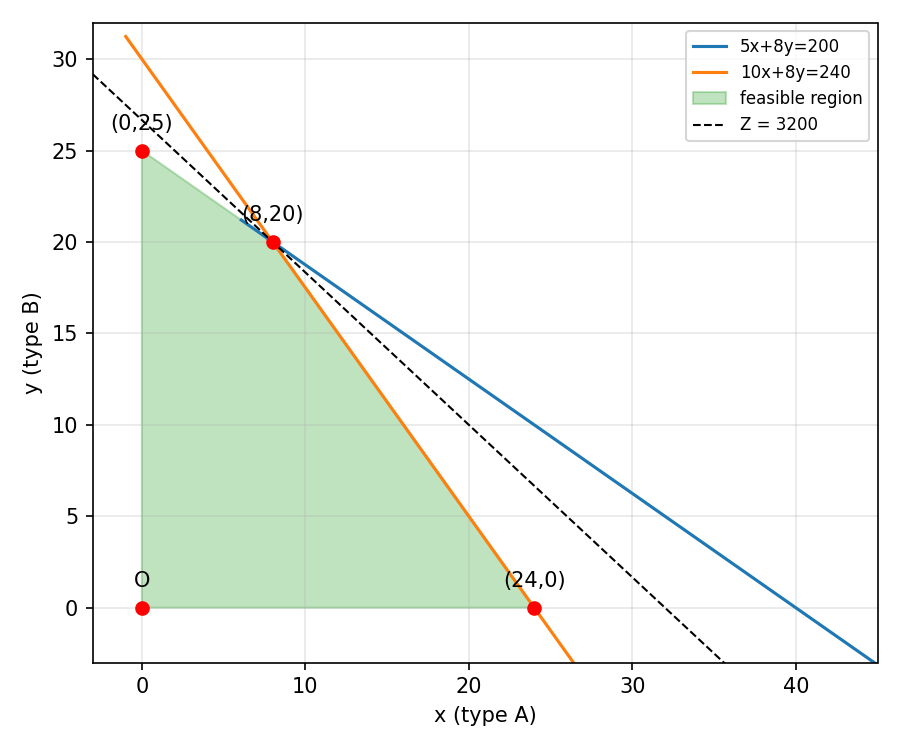
\includegraphics[width=0.70\linewidth]{figs/LPP.png}
    \caption{Feasible region and the optimum at $(8,20)$}
    \label{fig:lpp_q26}
\end{figure}

    \item
    \begin{enumerate}[label=(\alph*), leftmargin=1.5em, labelsep=0.5em]
        \item Find the vector equation of the line passing through $(2,1,-1)$ and parallel to the line $\vec{r} = (\hat{i}+\hat{j}) + \lambda(2\hat{i}-\hat{j}+\hat{k})$. Also, find the distance between these two lines.

        \begin{center}
            \textbf{OR}
        \end{center}

        \item Find the coordinates of the foot $Q$ of the perpendicular drawn from the point $P(1,3,4)$ to the plane $2x-y+z+3=0$. Find the distance $PQ$ and the image of $P$ treating the plane as a mirror.
    \end{enumerate} \vspace{2pt}
    \textbf{(a) Solution:} The required line has the same direction $\vec{b} = \myvec{2\\-1\\1}$ and passes through $\vec{a}_2 = \myvec{2\\1\\-1}$:
\begin{align}
    \vec{r} = (2\hat{i}+\hat{j}-\hat{k}) + \mu(2\hat{i}-\hat{j}+\hat{k})
\end{align}
With $\vec{a}_1 = \myvec{1\\1\\0}$, $\vec{a}_2-\vec{a}_1 = \myvec{1\\0\\-1}$ and
\begin{align}
    (\vec{a}_2-\vec{a}_1)\times\vec{b} = \myvec{0\cdot1-(-1)(-1) \\ (-1)(2)-1\cdot1 \\ 1\cdot(-1)-0\cdot2} = \myvec{-1 \\ -3 \\ -1}
\end{align}
From \eqref{eq:EE26BTECH11225-distance-lines}:
\begin{align}
    d = \frac{\sqrt{1+9+1}}{\sqrt{4+1+1}} = \sqrt{\frac{11}{6}} \approx 1.354\text{ units}
\end{align}
\textbf{(b) Solution:} The normal of the plane is $\vec{n} = \myvec{2\\-1\\1}$ and $c=-3$. From \eqref{eq:EE26BTECH11225-foot}:
\begin{align}
    t = \frac{-3-(2-3+4)}{4+1+1} = \frac{-6}{6} = -1
\end{align}
\begin{align}
    \vec{Q} &= \myvec{1\\3\\4} - \myvec{2\\-1\\1} = \myvec{-1\\4\\3} \\
    PQ &= |t|\,\|\vec{n}\| = \sqrt{6} \\
    \vec{P}' &= \vec{P}+2t\vec{n} = \myvec{1\\3\\4} - 2\myvec{2\\-1\\1} = \myvec{-3\\5\\2}
\end{align}
Thus $Q(-1,4,3)$, $PQ=\sqrt{6}$ and the image of $P$ is $P'(-3,5,2)$. The following code verifies both parts and generates \figref{fig:lines3d_q27}.
\begin{lstlisting}[frame=single, basicstyle=\rmfamily, escapeinside={(*@}{@*)}]
(*@\makebox[\dimexpr\linewidth-2\fboxsep-2\fboxrule\relax][c]{codes/Lines3D.py}@*)
\end{lstlisting}
\begin{figure}[H]
    \centering
    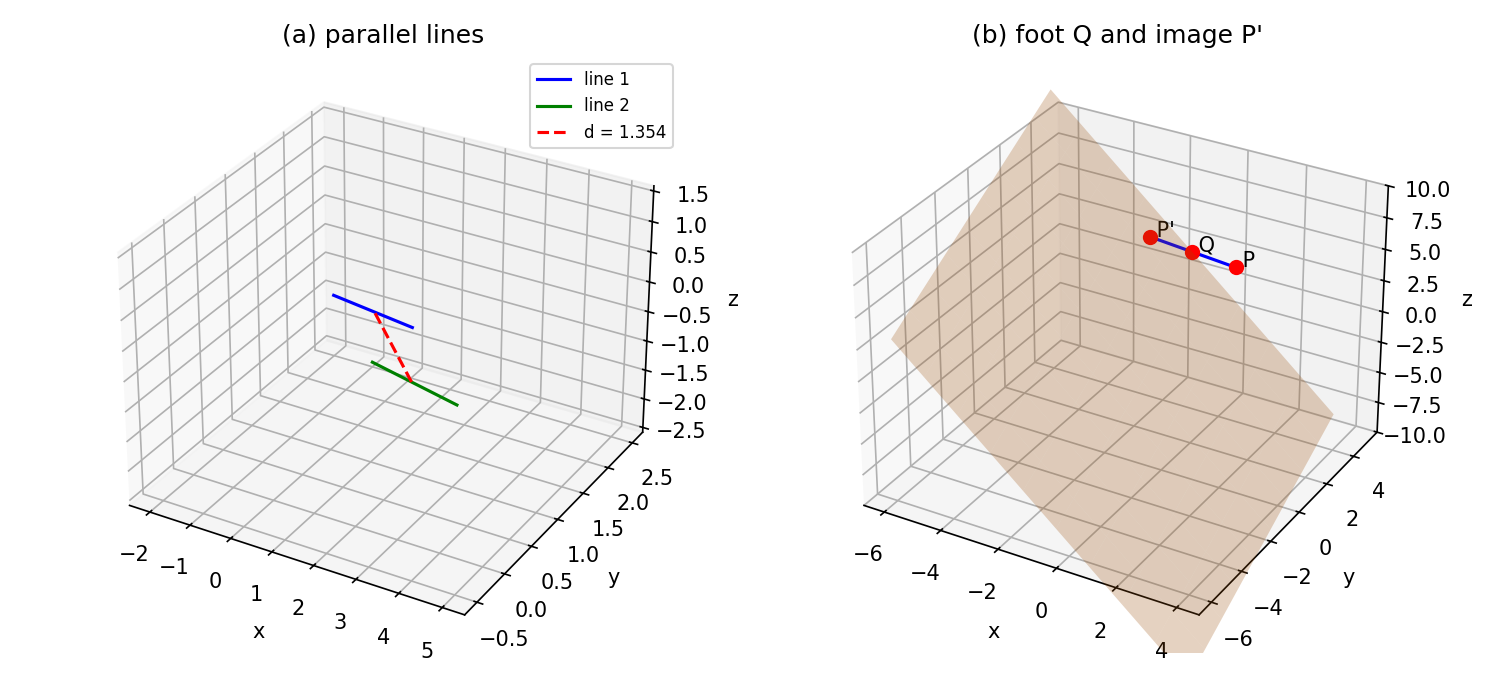
\includegraphics[width=0.95\linewidth]{figs/Lines3D.png}
    \caption{(a) The two parallel lines; (b) foot $Q$ and image $P'$ of $P$}
    \label{fig:lines3d_q27}
\end{figure}

    \item A card from a pack of 52 playing cards is lost. From the remaining cards of the pack, two cards are drawn at random (without replacement) and both are found to be spades. Find the probability of the lost card being a spade.

\solution Let $E_1$: the lost card is a spade, $E_2$: the lost card is not a spade, and $A$: both cards drawn are spades.
\begin{align}
    P(E_1) = \frac{13}{52} = \frac{1}{4}, \quad P(E_2) = \frac{3}{4}
\end{align}
If a spade is lost, 12 spades remain among 51 cards; otherwise 13 spades remain among 51 cards:
\begin{align}
    P(A|E_1) = \frac{12}{51}\cdot\frac{11}{50}, \quad P(A|E_2) = \frac{13}{51}\cdot\frac{12}{50}
\end{align}
From \eqref{eq:EE26BTECH11225-bayes},
\begin{align}
    P(E_1|A) &= \frac{\frac{1}{4}\cdot\frac{12\cdot11}{51\cdot50}}{\frac{1}{4}\cdot\frac{12\cdot11}{51\cdot50}+\frac{3}{4}\cdot\frac{13\cdot12}{51\cdot50}} \\
    &= \frac{132}{132+468} = \frac{132}{600} = \frac{11}{50}
\end{align}
The following code verifies the result with exact fractions and a simulation.
\begin{lstlisting}[frame=single, basicstyle=\rmfamily, escapeinside={(*@}{@*)}]
(*@\makebox[\dimexpr\linewidth-2\fboxsep-2\fboxrule\relax][c]{codes/Bayes.py}@*)
\end{lstlisting}

    \item Prove that the radius of the right circular cylinder of greatest curved surface area which can be inscribed in a given cone is half of that of the cone.

\solution Let the cone have base radius $R$ and height $H$, and let the inscribed cylinder have radius $r$ and height $h$. By similar triangles in the cross-section, from \eqref{eq:EE26BTECH11225-inscribed},
\begin{align}
    \frac{h}{H} = \frac{R-r}{R} \implies h = \frac{H(R-r)}{R}
\end{align}
The curved surface area is
\begin{align}
    S = 2\pi rh = \frac{2\pi H}{R}\left(Rr - r^2\right)
\end{align}
Differentiating,
\begin{align}
    \frac{dS}{dr} &= \frac{2\pi H}{R}(R-2r) = 0 \implies r = \frac{R}{2} \\
    \frac{d^2S}{dr^2} &= -\frac{4\pi H}{R} < 0
\end{align}
So $S$ is maximum at $r=\frac{R}{2}$, i.e. the radius of the cylinder is half the radius of the cone (and its height is $\frac{H}{2}$). Hence proved. The following code verifies the maximum and plots \figref{fig:cylinder_q29}.
\begin{lstlisting}[frame=single, basicstyle=\rmfamily, escapeinside={(*@}{@*)}]
(*@\makebox[\dimexpr\linewidth-2\fboxsep-2\fboxrule\relax][c]{codes/Cylinder.py}@*)
\end{lstlisting}
\begin{figure}[H]
    \centering
    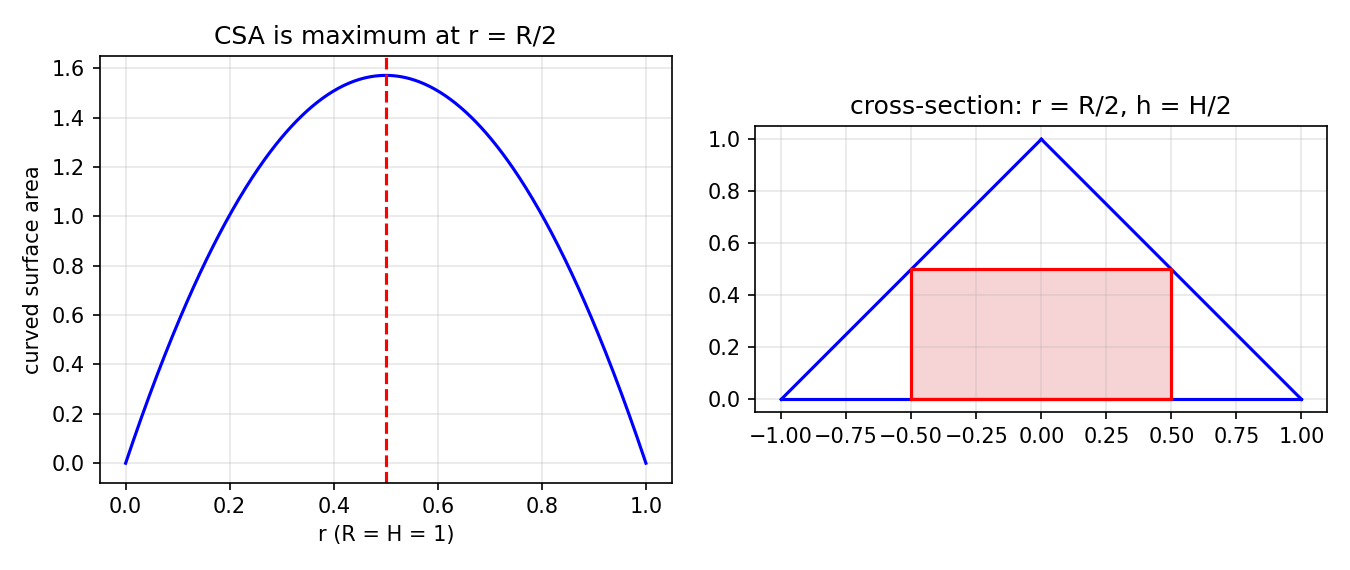
\includegraphics[width=0.95\linewidth]{figs/Cylinder.png}
    \caption{(a) Curved surface area against $r$; (b) the cylinder with $r=R/2$ inside the cone}
    \label{fig:cylinder_q29}
\end{figure}

\end{enumerate}

\end{document}
